\documentclass[smallextended]{svjour3}       % onecolumn (second format)

\clearpage{}\usepackage[T1]{fontenc}
\usepackage[utf8]{inputenc}
\synctex=-1 
\usepackage[english]{babel}

\usepackage[bookmarks=false, hidelinks]{hyperref} 
\usepackage{xspace}
\usepackage{multirow}
\usepackage[font=small]{caption}
\captionsetup{skip=4pt}

\usepackage{subcaption}
\usepackage{graphicx}
\usepackage{comment}
\usepackage{tabularx}

\usepackage[normalem]{ulem}
\usepackage{fixltx2e}
\usepackage{booktabs}
\usepackage{pslatex}
\usepackage[inline]{enumitem}
\usepackage{flushend}
\usepackage{tablefootnote}

\newcommand{\mytitle}{How the R Community Creates and Curates Knowledge:\\ A Comparative Study of Stack Overflow and Mailing Lists}
\newcommand{\myrunningtitle}{How the R Community Creates and Curates Knowledge}
\newcommand{\myauthor}{Zagalsky et al.}
\newcommand{\mysubject}{Q&A Knowledge curation}
\newcommand{\mykeywords}{Knowledge Curation, Case Study}

\hypersetup{pdftitle={\mytitle},
             pdfauthor={\myauthor},
             pdfsubject={\mysubject},
             pdfkeywords={\mykeywords}
}


\newenvironment{packed_enum}{
\begin{enumerate}[itemsep=3pt, topsep=2pt, leftmargin=2.4em, parsep=0pt]
}{\end{enumerate}}

\usepackage{color}
\usepackage{ifthen}
\newboolean{showcomments}
\setboolean{showcomments}{true}
\ifthenelse{\boolean{showcomments}}
  {
				\newcommand{\nbb}[2]{
				\fcolorbox{black}{yellow}{\bfseries\sffamily\scriptsize#1}
		{\sf$\blacktriangleright$\textcolor{blue}{\textit{#2}}$\blacktriangleleft$}
				}
        \newcommand{\dmg}[1]{{\color{blue}\emph{Daniel says: #1}}\xspace}
        \newcommand{\alexey}[1]{{\color{cyan}\emph{Alexey says: #1}}\xspace}
        \newcommand{\gpoo}[1]{{\color{red}\emph{Germán says: #1}}\xspace}
        \newcommand{\peggy}[1]{{\color{magenta}\emph{Peggy says: #1}}\xspace}
        \newcommand{\cassie}[1]{{\color{magenta}\emph{Cassie says: #1}}\xspace}
        \newcommand{\todo}[1]{\textcolor{red}{{\sc #1}}}
        \newcommand{\internalnote}[1]{\marginpar{\scriptsize note: #1}}
        \newcommand{\version}{\emph{\scriptsize{$-$\today$-$}}}
		\newcommand{\remarks}[1]{\color{red}[#1]\color{black}}
		\newcommand{\modified}[1]{\color{blue}[#1]\color{black}}
		\newcommand{\raw}{$\rightarrow$}
		\newcommand{\ins}[1]{\textcolor{blue}{\uline{#1}}} 		\newcommand{\del}[1]{\textcolor{red}{\sout{#1}}} 		\newcommand{\chg}[2]{\textcolor{red}{\sout{#1}}{\raw}\textcolor{blue}{\uline{#2}}} 		\newcommand{\ugh}[1]{\textcolor{red}{\uwave{#1}}} 		\newcommand{\cn}{\textcolor{blue}{[citation needed]}\xspace}
  }
  {
        \newcommand{\dmg}[1]{}
        \newcommand{\alexey}[1]{}
        \newcommand{\cassie}[1]{}
        \newcommand{\gpoo}[1]{}
		\newcommand{\nbb}[2]{}
        \newcommand{\todo}[1]{}
        \newcommand{\internalnote}[1]{}
		\newcommand{\remarks}[1]{}
		\newcommand{\modified}[1]{#1}
		\newcommand{\version}{}
		\newcommand{\ugh}[1]{#1} 		\newcommand{\ins}[1]{#1} 		\newcommand{\del}[1]{} 		\newcommand{\chg}[2]{#2} 		\newcommand{\cn}{}{}
  }

\newcommand{\channel}{communication channel\xspace}
\newcommand{\channels}{communication channels\xspace}
\newcommand{\Channel}{Communication channel\xspace}
\newcommand{\Channels}{Communication channels\xspace}

\newcommand{\SO}{Stack Overflow\xspace}
\newcommand{\RH}{R-help\xspace}

\newcommand{\rqa}{What types of knowledge artifacts are shared on Stack Overflow and the R-help mailing list within the R community?}
\newcommand{\rqb}{How is the knowledge constructed on Stack Overflow and the R-help mailing list?}
\newcommand{\rqc}{Why do users post to a particular channel and why do some post to both channels?}
\newcommand{\rqd}{How do users participate on both channels over time?}
\newcommand{\rqe}{Are there significant differences in participation activity between community users?}
%\newcommand{\rqd}{How have the communities of both Stack Overflow and the R-help mailing list evolved over time?}

\newcommand{\reca}{Choose the correct channel}
\newcommand{\recb}{Be aware of the channel rules and the basic concepts and nomenclature used}
\newcommand{\recc}{Provide good background to the question}
\newcommand{\recd}{Learn to use external resources}
\newcommand{\rece}{Behave altruistically}


\begin{document}



\title{\mytitle}

\author{
  Alexey~Zagalsky, Daniel~M.~German, Margaret-Anne~Storey, Carlos~Gómez~Teshima, Germán~Poo-Caamaño
}
\authorrunning{\myauthor}
\titlerunning{\myrunningtitle}

\date{\the\year}

\maketitle

\begin{abstract}
One of the many side effects of social media's prevalence in software development are the flourishing communities of practice where users share a common interest, such as programming languages, frameworks, and tools. These large communities use many different \channels but little is known about how they create, share, and curate knowledge using such channels.

In this paper, we report a mixed methods study of how one community of practice---the R software development community---creates and curates knowledge associated with questions and answers (Q\&A) in two of its main \channels: the R tag in Stack Overflow and the R-users mailing list. The results reveal that knowledge is created and curated in two main forms: participatory, where multiple users explicitly collaborate to build knowledge, and crowdsourced, where individuals primarily work independently of each other. Moreover, our study reveals participation patterns, showing the existence of prolific contributors: users who are active across both channels and are responsible for a large proportion of the answers, serving as a bridge of knowledge.

The key contributions of this paper are: a characterization of knowledge artifacts that are exchanged by this community of practice; the reasons why users choose one channel over the other; and insights on the community participation patterns, which indicate an evolution of the community and a shift from knowledge creation to knowledge curation. Finally, this paper enumerates a set of recommendations to assist practitioners in the use of multiple channels for Q\&A.
\end{abstract}

\section{Introduction}
\label{cha:introduction}

The emergence and adoption of socially enabled tools and channels
(e.g., GitHub, \SO, mailing lists) has fostered the formation of large
\textit{communities of practice} where users share a common
interest, such as programming languages, frameworks, and
tools~\cite{Storey2014}. These communities rely on many
different communication channels, but little is known about how
they create, share, and curate knowledge using such channels.

One prominent community of practice is the group that has formed in support of the R
programming language, an open source project without commercial
backing that relies heavily on its rapidly growing and highly
heterogeneous software development community. The R community plays an
important role in diffusing the R language: users have access to
numerous resources for learning the language and receiving help, such
as mailing lists, blogs, books, online and offline courses, and
question \& answer sites (e.g., \SO). While the R community benefits
from this vast and rich corpus of knowledge, it also drives the
creation and curation of the information.

Without a single entity directing and controlling it, the R language has grown organically from its community. Similar to other communities of practice, knowledge is exchanged and curated in many \channels, and two particular \channels are at the center of this process: the \textit{\RH mailing list} and \textit{\SO}. The \RH mailing list was created to assist those using the language, and while \SO is not specifically oriented towards R, its section dedicated to R (the R tag) has grown rapidly\footnote{\href{http://www.r-bloggers.com/r-is-the-fastest-growing-language-on-stackoverflow/}{http://www.r-bloggers.com/r-is-the-fastest-growing-language-on-stackoverflow/}}.

\SO has revolutionized the way programmers seek knowledge~\cite{li2013help,Vasilescu2014c}, assuming the role of a capable ``expert on call'' that is able---and willing---to answer questions of any level of difficulty about any programming technology (R included). \SO's gamification features guarantee that enthusiastic experts will answer questions, often within minutes of being posted~\cite{Mamykina2011}. Equally important is the ability of \SO's users to curate the knowledge being created, making sure that the best answers surface to the top and become a valuable asset to those seeking an answer now or in the future. \SO has become a popular and effective tool for creating, curating, and exchanging knowledge, including knowledge about the R language.

One would expect that the traffic on the \RH mailing list would begin
to fizzle as \SO popularity increased. If \SO is so effective at
matching those who seek knowledge with those that have it, doesn't
that obviate most of the need for the \RH mailing list? Yet that does
not appear to be the case as the \RH mailing list has maintained a
steady level of activity, implying that it is still an important resource for the R
community. It even appears as if the mailing list and \SO complement
each other.

There are obvious inherent differences between both \channels. On the one hand, mailing lists unite users by subscription, creating a tight community, but their content lacks organization, except for the natural structure provided by email metadata (e.g., subjects, threading, authors, dates), and they are not optimized for long-term storage and retrieval. On the other hand, \SO's community is not as tight as an email community, but the channel is optimized for the curation and long-term storage of knowledge. However, little is known about the differences in how people use both \channels, such as how the types of questions and answers sought in one channel compare to the other, why users choose one channel over the other, why some users participate in both channels, and how participants perceive each \channel.



In this paper, we empirically compare how
knowledge, specifically knowledge manifested as questions and answers,
is sought, shared, and curated on both the \RH mailing list and
\SO.  We also review the participation patterns of users in both
communities. 
Our research employed a mixed methods \textit{exploratory case study}
methodology to answer the following research questions:

\begin{enumerate}[label=\bfseries{RQ\arabic*.},itemsep=3pt, topsep=2pt, leftmargin=3em, parsep=0pt]
\item \rqa
\item \rqb
\item \rqc
\item \rqd
\item \rqe
\end{enumerate}

By mining archival data, we identified and categorized the main types
of knowledge artifacts contained on the \RH mailing list and in \SO
messages (RQ1). The emerging categories form a \textit{typology} (see
Table~\ref{table:type-of-knowledge}) that
allows researchers to study and characterize Q\&A knowledge
dissemination within a community of practice. We used this typology to
study how knowledge is constructed and shared on \SO and the \RH
mailing list. We found that these channels support two distinct
approaches for constructing knowledge---\textit{participatory
  knowledge construction} and \textit{crowd knowledge
  construction}---however, each channel supports them differently
(RQ2). Our findings indicate that participatory knowledge construction
is more prevalent on the \RH mailing list, while crowd knowledge construction is more
prevalent on \SO.

We found that some contributors are active on both channels. As a
result, we conducted a survey to investigate the benefits they gain by
doing so (RQ3). But beyond that, we wanted to examine how participation differs between \SO and the \RH mailing list over time and how long users participate on the two channels (RQ4). Additionally, we wanted to understand the behavior and \textit{participation patterns} of the contributing users (RQ5). We focused on several sets of contributors: those who rarely contribute,
the top contributors, and those who contribute to both channels. 
Our results show that a great majority of participants are
fleeting and a small number of individuals are responsible for most
answers.  Furthermore, our findings indicate that both channels are reaching
maturity: for the \RH mailing list, this means a steady flow of questions; for \SO, there is a continuous decrease of questions with a positive score
(number of positive votes minus negative votes), hinting to the fact
that, as time progresses, the most frequently asked questions have
been already asked.

We conclude the paper by providing recommendations for
using the different communication channels, and discussing how channel
affordances and community rules (e.g., topic restriction and
gamification) influence knowledge construction and curation.

 \section{Background}
\label{cha:background}
We begin with an overview of the R community and detail the two main channels its users use to ask and answer questions.

\subsection{The R Community of Practice}
    
    The R project\footnote{\url{https://www.r-project.org/}} was born in 1993 as a free and open source programming language and software environment for statistical computing, bioinformatics, and graphics~\cite{Ihaka1996}.
    The R community is composed of:
    \begin{enumerate*}[label=(\arabic*)]
      \item \textit{R-core}, a team of 20 software developers that maintain and evolve the R language; and
      \item \textit{Periphery}, which includes everyone else (language users and package developers).
    \end{enumerate*}

    The R community is an eclectic open source community that goes beyond software development 
    and includes biologists and statisticians with no or limited programming experience.
    Its entire history of mailing list communication is archived and publicly available.
    The R community has also been the subject of extensive research in community evolution~\cite{German2013,Vasi1escu2014PhD} and the interplay between channels~\cite{Vasilescu2014c}.

    R's popularity has continuously increased over the years. 
    IEEE Spectrum recently ranked R as the 5th most popular
    language\footnote{\url{http://spectrum.ieee.org/computing/software/the-2016-top-programming-languages}},
    implying that the R community is healthy and continues to grow at
    a fast rate.

    Our study focused on the analysis of \SO and the \RH mailing list, two channels in the R community.
    We chose them because they are the main channels that provide Q\&A support to the community.

\subsubsection{R-help Mailing List}
    There are several mailing lists to help R community users solve programming problems with the R language: \emph{R-help}, \emph{R-package-devel}, \emph{R-devel}, \emph{R-packages}, \emph{R-announce}, and \emph{Bioconductor}. However, the \RH mailing list is the main channel for discussing problems and solutions using R. Other messages are also encouraged, such as documentation, benchmarks, examples, and announcements.

    The \RH mailing list used to be the main \channel for asking
    and answering questions within the R community, but a significant
    number of users migrated to \SO~\cite{Vasilescu2014c}.
    Despite the reduced number of users, the \RH mailing list is
    still very active---on average, a subscriber may receive
    approximately 30 emails
    a day (as of Oct 2016).

\subsubsection{Stack Overflow}
\label{subsec:Rtag}

    In contrast to the \RH mailing list, \SO incorporates a rich visual and user-friendly interface with social media and gamification features.
    The social aspect of the Website improves participation and provides strong support for creating and sharing knowledge as well as encouraging informal mentorship~\cite{Jenkins2009,Storey2014}.
    Meanwhile, \SO's gamification features provide reputation points and badges to reward user participation and earn them points that enable functionality inside the site.
    It has been reported that \SO's gamification mechanisms boost participation~\cite{Vasi1escu2014PhD} and enable mutual assessment~\cite{Singer2013}.


\subsection{\SO vs. Mailing Lists}
Software development is a knowledge-building process~\cite{naur1985programming}. Due to the emergence of socially enabled tools and channels and the formation of communities of practice~\cite{Storey2014}, it is important to understand how knowledge is created and shared within these communities. In our study, we focus on knowledge in the form of questions and answers within the R community.


As part of a study on the transition to gamified environments, Vasilescu~\cite{Vasi1escu2014PhD} examined the popularity of Stack Exchange (including the \SO R tag) and
mailing lists within the R community. He found that the number of message threads has decreased on the \RH mailing list since 2010, while the number of
R-related questions asked on the Stack Exchange network has increased. Our study also examined \SO's R tag and the \RH mailing list, but we aimed to understand the \textit{knowledge types} used. This allowed us to characterize the different knowledge seeking and sharing approaches on each channel. Vasilescu also examined the \textit{difference in activity} between contributions made by users active on both channels and users focused on a single medium. While we also found users of the R community that were active on both channels, we aimed to understand \textit{why users post to a particular channel}.
\alexey{we may need to adjust the previous sentence comparing our study with Vasilescu, since we plan to add similar type of analysis in the extension.}

Similar to Vasilescu, Squire~\cite{Squire2015a} studied a project's \textit{transition to the \SO gamified channel}. She focused on examining whether four software projects that moved from mailing lists to \SO showed improvements in terms of developer participation and response time. She found that all four projects showed improvements on \SO compared to mailing lists, however, she also found that several projects have moved back to using mailing lists despite achieving these improvements. In our study, we found that both channels have knowledge support for question and answers, however, there are important differences between the two channels. For example, \SO's competitive environment creates an incentive to be the first to answer rather than improve other answers and participate in discussions.

\section{Methodology}
\label{cha:methodology}

As mentioned, the main goal of this work is to empirically compare how knowledge, specifically knowledge in question-and-answer (Q\&A) form, is sought, shared, and curated on both the \RH mailing list and the R tag on \SO. We used a mixed methods \textit{exploratory case study} methodology~\cite{Creswell2009,Runeson2012} to answer our research questions (presented in Section~\ref{cha:introduction}).
                    
This study employed two research methods over three phases: we \textit{mined archival data} and then conducted a \textit{qualitative survey}. In the first phase, we randomly sampled and iteratively coded\footnote{Our sample data is openly available at \url{https://github.com/thechiselgroup/R-ML-and-StackOverflow}} questions in both channels to characterize the types of discussions that occur. This process was continued until we reached saturation, which amounted to 400 threads in each channel. In the second phase, we surveyed users of the R community to validate our interpretation of the results from the previous phase. And in the third phase, we extended the collected data set up to September 2016 and focused on investigating participation patterns on both channels.

\subsection{Phase I: Mining Archival Data} 
\label{sec:studyDesign}

We mined data from the public archives of both the \RH mailing list and \SO. The \RH mailing list archive started in 1997, while the archives for \SO started in 2008 (when it was created).
To make the data sets comparable, we analyzed both datasets from September 2008 until December 2013, a period of time that both channels were available.
For \SO, we obtained a data dump file from their Website---Stack Exchange releases a new data dump from all their Websites every three months\footnote{\url{http://stackexchange.com/sites}}. For the \RH mailing list data, we retrieved MBOX files of the archives from the \RH Website.

To answer RQ3, we also needed the ability to compare email addresses between both channels. However, Stack Exchange stopped providing information about email addresses---the last Stack Exchange dump file to contain email addresses as MD5 hashes was released in September 2013, so this meant we did not have complete data for October, November, and December 2013. To remedy this gap, we used the data dump file from September 2014, but updated the \texttt{users} table with the hashes taken from the September 2013 dump file for those \texttt{ID}s that were identical in both data sets. If a user in the 2013 data file did not exist in the 2014 data, we did not examine them. From \SO, we retrieved all R-related data by selecting only messages that contained the R tag (\texttt{r}) or its two synonyms\footnote{\url{http://stackoverflow.com/tags/r/synonyms}},
(\texttt{rstats} and \texttt{r-language}).

To determine which users were active in both channels, we compared the MD5 hashes of the email addresses extracted from the \RH mailing list and \SO. If there was match, we associated the \RH and \SO user accounts to the same person. Using this approach, we identified 1,421 persons who used both media channels.

To prepare the data, we used two different software tools:
    \begin{enumerate*}[label=(\arabic*)]
    \item To process the \SO data, we used a modified version of Sam Saffron's application, So-Slow\footnote{\url{https://github.com/SamSaffron/So-Slow}}.
    \item To process the \RH mailing list data, we wrote our own mail mining application\footnote{Our tool is available at
            \url{https://github.com/cagomezt/GTMail}}. To ensure accurate results when processing the \RH mailing list, we followed a series of recommendations proposed by Bettenburg \textit{et al.}~\cite{Bettenburg2009}: extracted messages, removed duplicates, removed signatures, and reconstructed discussion threads.
    \end{enumerate*}
Table~\ref{table:data} depicts a summary of the data used for this study. Unsurprisingly, the \RH mailing list has more questions, answers, and users as it contains approximately ten years of additional data.
Note that only \SO's data contains ``comments'' information.

	\begin{table}[!htb]
	  \centering
      \caption{Raw data collected for each channel during Phase I - up to September 2014.}
      \begin{small}
        \begin{tabular}{lrr}
	        \toprule
	        Type          &  \RH & \SO \\
	        \midrule
	        Questions     & 101,931 &  67,393 \\
	        Answers       & 213,366 &  99,620 \\
	        Comments      &       - & 286,124 \\
          Different individuals & 31,729 &  26,324 \\
	        \bottomrule
        \end{tabular}
      \end{small}
	  \label{table:data}
	\end{table}

\subsubsection{Data analysis process}
\label{sec:dap}

We followed an inductive approach~\cite{Runeson2012} to analyze the data from \SO and the \RH mailing list. To reduce the risk of bias~\cite{Runeson2012}, the analysis was conducted by two computer scientists with a background in qualitative data analysis. To answer RQ1 and RQ2, we selected 400 random threads from each channel. To answer RQ3, we focused on questions with identical subjects that were posted to both channels by the same author---we found and analyzed 79 such threads.

\begin{figure*}[htbp]
	\centering
	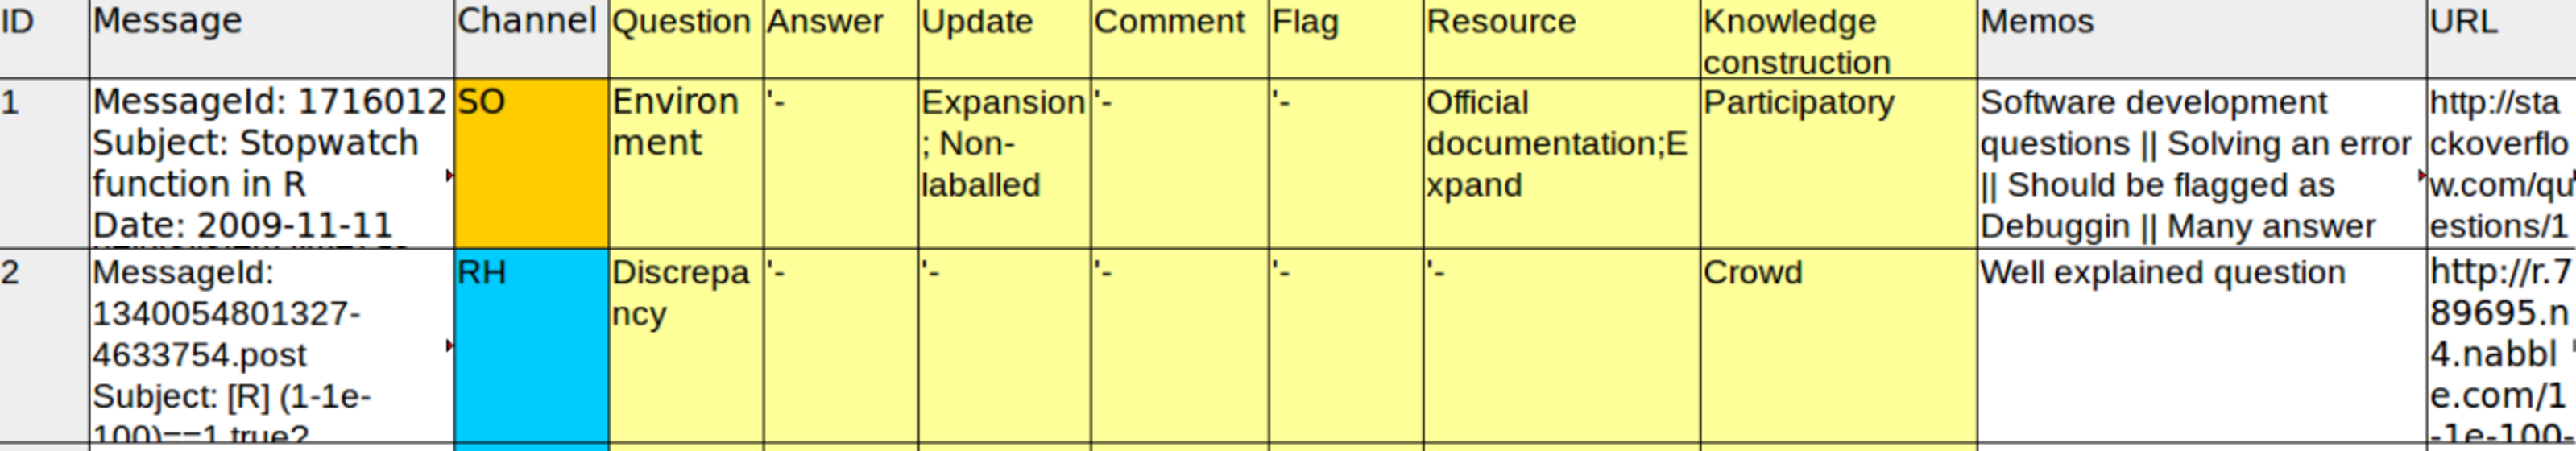
\includegraphics[width=.95\textwidth]{../Figures/CodingExample}
	\caption{Example of data coding. Each row is a threaded message. Questions, comments, and answers are identified with the number on the first column. Columns in yellow (columns 4-10) contain the code for each message type. The last two columns contain the memos and URLs.}
	\label{fig:CodingExample}
\end{figure*}

We used memoing, affinity diagrams, and a code book to support the data analysis process. We wrote reflective memos in a spreadsheet next to the applicable codes (see example in Fig.~\ref{fig:CodingExample}). These memos were used to create the codes and hypotheses about the relationships between concepts. We coded in multiple sessions, which allowed us to refine the definitions in the code book iteratively. Each entry is associated with a title, a formal definition, an example, and notes from the researchers. For inter-rater reliability, we used the Cohen Kappa inter-rater agreement coefficient~\cite{Stemler2004}. Although it is suggested that one should aim for coefficient values above 0.6 to obtain substantial results~\cite{Landis1977}, based on our previous experience with this method~\cite{Gomez2013}, we aimed for 0.8 or above. We used this coefficient after each coding session as a way to trigger discussion and to further refine the codes if necessary.  
The emergent codes were fully saturated after reviewing 400 threads from each channel.


The analysis process required an \textit{understanding of the context} surrounding each message. The process consisted of: (1) gathering the required information from each channel (i.e., the message analyzed, the relevant thread), and (2) mapping the messages from each channel to a specific knowledge type (see Section~\ref{cha:findings-types}). The mapping was necessary as each channel contained a different data structure.
We defined the following mappings between messages in both channels:

	\begin{description}[itemsep=1pt, topsep=2pt, leftmargin=1em, parsep=0pt]
		\item[\textbf{Question:}] The message is the first in the thread and contains the main question.
		\item[\textbf{Answer:}] The message provides a solution to the main question of the thread.
	 	\item[\textbf{Update:}] The message requests a modification to a question or answer made by the author of said question or answer.
		\item[\textbf{Comment:}] The message offers clarification to a specific part of the question or answer.
		\item[\textbf{Flag:}] The message requests attention from the moderator (e.g., repeated questions, spam, or rude behavior).
	\end{description}


\subsection{Phase II: Qualitative Survey}

The analysis from Phase I revealed that some developers are active on both channels, and in some cases, even post the same questions. To further understand this phenomena and explore the perceived benefits of using one channel over the other, we conducted a survey with users of the R community\footnote{A copy of the survey is available at \url{http://goo.gl/mxmH5J}}. 
To test and refine the questions, format, and tone, we piloted the survey twice. 
We promoted our survey on Twitter, Reddit, the \RH mailing list, and Meta Stack Exchange to reach users of both channels and minimize selection bias. However, our survey invitation on Stack Exchange was deemed off topic and deleted a few minutes later. In total, we received 37 responses, 26 of which were valid (invalid responses occurred if the session ended or the participant did not complete the survey).

\subsection{Phase III: An Extended Quantitative Analysis}

In this phase, we focused our analysis on the behavior and participation patterns of community users on the \RH mailing list and \SO. We extended our analysis to include archival data from September 2008 up to September 2016 for both channels. 

For \SO, we used Stack Exchange's Data Explorer\footnote{\url{https://data.stackexchange.com/stackoverflow/query/new}} to query the data. The structured metadata allowed us to automatically classify each message as a question, an answer, or a comment.

For the \RH mailing list, we downloaded all the email threads and extracted the separate emails and corresponding metadata from each thread. As opposed to \SO, the \RH mailing list data doesn't include metadata to indicate whether a message is a question or an answer. Thus, we used the following heuristic to classify the \RH messages: if a message contained an \texttt{In-Reply-To} or a \texttt{References} header, it was classified as an answer (239,976 responses); otherwise, a message was classified as a question (124,925 questions).

To study the participation behavior of different users, we assigned them a unique \texttt{person} identifier and performed a unification of identities. We extracted email addresses from the \RH mailing list data using the \texttt{From:} field, and using a conservative approach, identified messages sent by the same person but from different email addresses. As a result, the number of unique individuals identified on \RH was reduced from 36,600 to 31,731 (a reduction of 15\%)---a similar number was reported by Vasilescu \textit{et al.}~\cite{Vasilescu2014c}. Next, by using MD5 hashes of the email addresses extracted from the \RH mailing list and \SO, we identified 1,480 persons who used both media channels. We summarize the data collected during this phase in Table~\ref{table:extended_data}.

\begin{table}[!htb]
  \centering
    \caption{Raw data collected for each channel during Phase III - up to September 2016.}
    \begin{small}
      \begin{tabular}{lrr}
        \toprule
        Type          &  \RH & \SO \\
        \midrule
        Questions     & 101,931 &  67,393 \\
        Answers       & 213,366 &  99,620 \\
        Comments      &       - & 286,124 \\
        Different individuals\tablefootnote{Note: \SO data about user activity only goes up to September 2014.} & 31,729 &  26,324 \\
        \bottomrule
      \end{tabular}
    \end{small}
  \label{table:extended_data}
\end{table}



 \section{Findings}
\label{cha:findings}
In this section, we present our findings.
To understand how knowledge in the form of questions and answers is created, shared, and curated, we first identified and categorized the main types of knowledge artifacts contained within \RH mailing list messages and in \SO messages with the R tag (RQ1). The emerging categories formed a typology and allowed us to identify and describe two approaches for constructing knowledge that are supported by these channels (RQ2). Interestingly, we found that some developers are active on both channels, and in some cases, even post the same questions. As a result, we investigated the benefits they gain by doing so (RQ3). We also present our findings about participation on the two channels over time (RQ4) and look closely at differences on participation activity between community users (RQ5). \alexey{add RQ4-about the extension.} 

% RQ1
\subsection{What Types of Knowledge Artifacts Are Shared on \SO and the \RH Mailing List}
\label{cha:findings-types}

To answer RQ1, we randomly sampled 400 threads of messages from both \SO and the \RH mailing list, where each thread included a question and the associated responses. We identified five main types of artifacts that capture knowledge:
\begin{enumerate*}[label=(\arabic*)]
\item Questions, 
\item Answers,
\item Updates,
\item Flags, and
\item Comments.
\end{enumerate*}
Through our analysis, we further divided these types into sub-types---Table~\ref{table:type-of-knowledge} presents our typology of knowledge artifacts, their
descriptions, and their frequency in the sample of 400 threads in each channel. Even though we did not aim for a statistically significant sample size, the size of this sample
(400 threads in each channel) guarantees a confidence level of approximately 95\% $\pm$ 5\% for both channels. Using the Chi-square test of independence, we tested whether the distribution of types and sub-types of questions were different between the two channels.  In
all cases, they were found to be statistically different (with $\rho \ll 0.001$ in all cases).
    \begin{table*}[!htb]
      \centering
      \caption{Typology of knowledge artifacts found on both \SO (SO) and the \RH (RH) mailing list and their frequency in the analyzed sample. Numbers in bold represent the most significant differences between the two sets.}
      \begin{small}
\begin{tabular}[h]{p{2.3cm}p{10.3cm}rrrrr}
 && \textbf{SO}                                                                                                                                              & \textbf{RH}  & \textbf{Prop SO} & \textbf{Prop RH}                \\
\toprule
\multicolumn{2}{@{}l}{\textbf{Questions}}\\
  \emph{How-to}                   & Asks how to do something specific.                                                                                                                        & {166}          & {103}              & \textbf{41.50\% }       & \textbf{25.75\%}        \\
  \emph{Bug/Error\-/Exception}    & Asks for a solution or reasons for an error message.                                                                                                       & 27           & 48               & 6.75\%         & 12.00\%        \\
  \emph{Discrepancy}              & Asks about an unexpected result of a specific function, process, or package.                                                                              & 53           & 88               & \textbf{13.25\%}        & \textbf{22.00\%}        \\
  \emph{Set-up}                   & Asks for possible ways to set up the R environment before or after deployment.                                                                            & 15           & 31               & 3.75\%         & 7.75\%         \\
  \emph{Decision help}            & Asks for advice in making a decision.                                                                                                                     & 36           & 35               & 9.00\%         & 8.75\%         \\
  \emph{Conceptual\-/Guidance}    & Asks for conceptual clarification or guidance on topics related to R or statistics.                                                         & 48           & 49               & 12.00\%        & 12.25\%        \\
  \emph{Code reviewing}           & Asks for a code review, explicitly or implicitly.                                                                                                           & 34           & 21               & 8.50\%         & 5.25\%         \\
  \emph{Non-functional}           & Asks for help (or suggestions) with a non-functional requirement such as performance or memory usage.                                                   & 14           & 11               & 3.50\%         & 2.75\%         \\
  \emph{Future reference}         & Asks a question (often self-answering it) that might not exist on the channel, but that is interesting enough to warrant a thread for future reference.         & 5            & 4                & 1.25\%         & 1.00\%         \\
  \emph{Other}                    & Asks for assistance unrelated to the channel, or the message contains unrelated information (e.g., announcements, ideas for improvement).                  & 2            & 10               & 0.50\%         & 2.50\%         \\\cline{3-6}
                                  &                                                                                                                                                          & {400} & {400}     & {100\%} & {100\%} \\
\hline
  \multicolumn{2}{@{}l}{\textbf{Answers}}                                                                                                                                                                                                                          \\
  \emph{Redirecting}                & Provides a link to an existing solution that is not in the thread (e.g. external application, tutorial, project).                                     & 163          & 87               & 20.20\%        & 15.03\%        \\
  \emph{Tutorial}                   & Provides a set of steps to teach people how to solve the issue.                                                                                          & 105          & 15               & \textbf{13.01\%}        & \textbf{2.59\% }        \\
  \emph{Source code}                & Provides a source code snippet as the solution without an extensive explanation about the answer.                                                                   & 198          & 102              & 24.54\%        & 17.62\%        \\
  \emph{Clue/Suggestion/Hint}       & Provides a possible way(s) to fix the issue without actually solving it.                                                                                                     & 43           & 105              & \textbf{5.33\% }        & \textbf{18.13\% }       \\
  \emph{Alternative}                & Provides a different approach to a solution that is related to but not exactly what is being asked (e.g. mathematical approach, data structure modification). & 33           & 98               & \textbf{4.09\% }        & \textbf{16.93\% }       \\
  \emph{Explanation}                & Provides an explanation of an approach that answers the question and lists steps on how to do it.                                                                          & 203          & 101              & 25.15\%        & 17.44\%        \\
  \emph{Announcement}               & Provides a notification about some artifact (e.g., packages, libraries).                                                                                 & 8            & 33               & 0.99\%         & 5.70\%         \\
  \emph{Benchmark}                  & Provides a benchmark of multiple solutions posted by others or compares different answers.                                                               & 5            & 3                & 0.62\%         & 0.52\%         \\
  \emph{Opinion}                    & Provides an opinion or an expansion of another answer by including scenarios and examples.                                                                    & 49           & 35               & 6.07\%         & 6.04\%         \\\cline{3-6}
                                    &                                                                                                                                                          & \textbf{807} & \textbf{579}     & {100\%} & {100\%} \\
\hline
  \multicolumn{2}{@{}l}{\textbf{Updates}}                                                                                                                                                                                                                          \\
  \emph{Announcement}               & Announces specific events (e.g., bounties, future updates).                                                                                              & 27           & 3                & 4.40\%         & 1.21\%         \\
  \emph{Background}                 & Adds additional context to the question or answer .                                                                                                       & 74           & 57               & 12.07\%        & 23.08\%        \\
  \emph{Correction}                 & Corrects format, grammar, spelling, and semantic mistakes.                                                                                               & 301          & 2                & \textbf{49.10\% }       & \textbf{0.81\% }        \\
  \emph{Expansion}                  & Expands the question or answer by providing scenarios or examples.                                                                                       & 116          & 83               & \textbf{18.92\% }       & \textbf{33.60\%}        \\
  \emph{Explanation}                & Explains or clarifies a specific point in the question or answer, such as why the user chose a specific data structure, or the meaning of a variable.    & 83           & 95               & 13.54\%        & 38.46\%        \\
  \emph{Solution}                   & The user answers their own question.                                                                                                                     & 12           & 7                & 1.96\%         & 2.83\%         \\\cline{3-6}
                                    &                                                                                                                                                          & \textbf{613} & \textbf{247}     & {100\%} & {100\%} \\
\hline
  \multicolumn{2}{@{}l}{\textbf{Flags}}                                                                                                                                                                                                                            \\
        \emph{Off-topic/Opinion}          & Identifies questions that are unrelated to the channels' interests or requests answers based on opinion.                                                      & 22           & 19               & 27.16\%        & 35.19\%        \\
      \emph{Not an answer}              & Indicates answers that are out of scope of the question, or that do not answer the question.                    & 0            & 27               & \textbf{0.00\% }        & \textbf{50.00\%}        \\
    \emph{Repeated question}          & Notifies a user that the question has been answered previously.                                                                                                & 48           & 8                & \textbf{59.26\%}        & \textbf{14.81\%}        \\
  \emph{Too localized}              & Questions that are too specific and might not help future readers.                                                                                    & 6            & 0                & 7.41\%         & 0.00\%         \\
  \emph{Unclear}                    & Questions that are difficult to understand.                                                                                                              & 5            & 0                & 6.17\%         & 0.00\%         \\\cline{3-6}
                                    &                                                                                                                                                          & {81}  & {54}      & {100\%} & {100\%} \\
\hline
  \multicolumn{2}{@{}l}{\textbf{Comments}}                                                                                                                                                                                                                     \\
  \emph{Clarification}          & Provides (or requests) additional information about a question or answer.                                                                                & 98           & 28               & 17.44\%        & 10.49\%        \\
  \emph{Expansion}              & Provides additional information.                                                                                                                         & 127          & 65               & 22.60\%        & 24.34\%        \\
  \emph{Correction/Alternative} & Suggests a change to a question or answer, offers an alternative solution or a correction.                                                               & 102          & 89               & \textbf{18.15\%}        & \textbf{33.33\% }       \\
  \emph{Compliment/Critic}   & Posts something good, offers thanks, or provides an opinion or criticism.                                                                           & 157          & 52               & 27.94\%        & 19.48\%        \\
  \emph{External reference}     & References an external resource.                                                                                                                         & 78           & 33               & 13.88\%        & 12.36\%        \\\cline{3-6}
                                &                                                                                                                                                          &{562}  & {267}     & {100\%} & {100\%} \\
  \bottomrule
        \end{tabular}
      \end{small}
      \label{table:type-of-knowledge}
\vspace{-3mm}
    \end{table*}

\paragraph{Questions and Answers}
    Questions express one or more problems or concerns faced by a user on the \RH mailing list or on \SO, whereas answers represent solutions to questions.  We observed that the types of questions on \SO are more specific than those on the \RH mailing list, and \SO answers are more likely to be tutorials. Also, \SO has more answers per question---2 per question compared to 1.4 for \RH (see Table~\ref{table:type-of-knowledge}). However, \RH answers tend to offer more suggestions or alternatives than \SO answers. 
\paragraph{Updates}
An update is a modification of a question or answer. In \SO, updates are presented in one of two ways.
\begin{description}[itemsep=3pt, topsep=2pt, leftmargin=1em, parsep=0pt]
\item[\textbf{Labeled updates}] are explicitly shown in the body of questions or answers next to a label that identifies the update (e.g., edit, update, and p.s.).
  When multiple update labels appear in a message, each label is accompanied by a number (e.g., \textit{``[Edit 1:]''}), a date (e.g., \textit{``Edit/Update (April 2011):''}), or a bulleted list
  (e.g., ``EDIT: - anova... -drop1...'').
\item[\textbf{Non-labeled updates}] are only visually recognizable through the message history system. The only indication of the change is a box at the end of the message that identifies the user who performed the change and the date when it occurred.
\end{description}
We found that non-labeled updates are often used to correct formatting, grammar, semantic mistakes, and spelling, or to incorporate explanations, examples, and suggestions without changing the meaning of the question or answer. Labeled updates are for everything else.

On the \RH mailing list, all communication occurs through emails, and authors do not explicitly tag messages as updates. For this reason, we define an update on \RH as \emph{a message sent to a thread where the author has already participated once}.

Regarding update frequency in our sample, the \SO R tag contained 2.5 more updates than the \RH mailing list. Corrections are more common on \SO (almost 50\%), while \RH updates are often related to the adding of information to a thread (providing background, expansion, and explanation).

\paragraph{Flags}
Flags are used to alert users of the community that a question or answer does not match community expectations.
%
\SO contains a flagging mechanism, often used to get a moderator's attention. These flags can accomplish various objectives: mark a message as containing spam or rude/abusive behavior, or identify
duplicate questions, off-topic messages, unclear questions, opinion-based questions, and low-quality
answers. Depending on the type of flag, this can lead to a thread being closed or the loss of user reputation points.  

The \RH mailing list doesn't have a built-in flagging mechanism, however, \RH users utilize the concept of flags, which we define as \emph{messages used to call the attention of other community users}, similar to the way flags are used in \SO.
%
In terms of their frequency, R tag posts on \SO contained 1.5 times more flags than posts on the \RH mailing list. \SO flags are primarily used to mark repeated questions. In contrast, flags on \RH are often used to indicate that a previous answer is incorrect.

\paragraph{Comments}

In \SO, comments are considered ``temporary `Post-It' notes left on a question or answer''\footnote{\url{http://stackoverflow.com/help/privileges/comment}}. Comments are located below each question or answer and can be used as a follow-up to a question, or to answer or clarify a question. On the \RH mailing list, we define comments as messages written to \emph{improve an answer or as a follow-up to a discussion}. It should be noted that in order for an email to qualify as a comment, it should not be written by the person who asked or answered the original question (otherwise, the message would be considered an update).
Because both \SO and the \RH mailing list permit participants to ask multiple questions in the same thread, the sub-categories of comments are not mutually exclusive.  

Regarding the frequency of comments, the main difference between the two channels is that \SO comments are less likely to be considered corrections or alternatives (Correction/Alternative sub-category) than on the \RH mailing list. The \SO R tag sample also contained 2.1 times more comments than the \RH sample (see Table~\ref{table:type-of-knowledge}).

% RQ2
\subsection{How Knowledge Is Constructed on \SO and the \RH Mailing List}
\label{sec:rq2}

Our analysis helped us identify two different approaches used for constructing knowledge (RQ2) on \SO and the \RH mailing list: participatory knowledge construction and crowd knowledge construction.

\begin{description}[itemsep=2pt, topsep=0pt, leftmargin=1em, parsep=0pt]
\item[\textbf{Participatory knowledge construction}] is an approach where answers are created through the cooperation of multiple users in the same thread. Participants complement each other's solutions by discussing the pros and cons of each answer, and by adding different viewpoints, additional information, and examples. This process is similar to a team working together towards a common objective.

\item[\textbf{Crowd knowledge construction}] leverages the experiences of many users who work in a relatively independent manner. Each user contributes to the thread, adding variety to the pool of solutions. However, the user's priority is to provide a correct answer and not to discuss other solutions. This is comparable with the concept of a group in which people work towards the same objective but not necessarily together (e.g., Amazon's Mechanical Turk). Participants can vote on other's ideas, but the main idea is not constructed through a discussion process.
\end{description}

On the \RH mailing list, \textit{participatory knowledge} construction takes place when:
\begin{enumerate*}[label=(\arabic*)]
  \item previous answers are included in the current answer with clear links between them; or
  \item a reply contains a direct reference to other answers or authors.
\end{enumerate*}
Figure \ref{fig:ML-PK1} depicts two examples of the way participatory knowledge occurs on the \RH mailing list: direct citation of the author of a previous answer, and inferable links between answers.

    
    \begin{figure}[!htb]
        \centering
        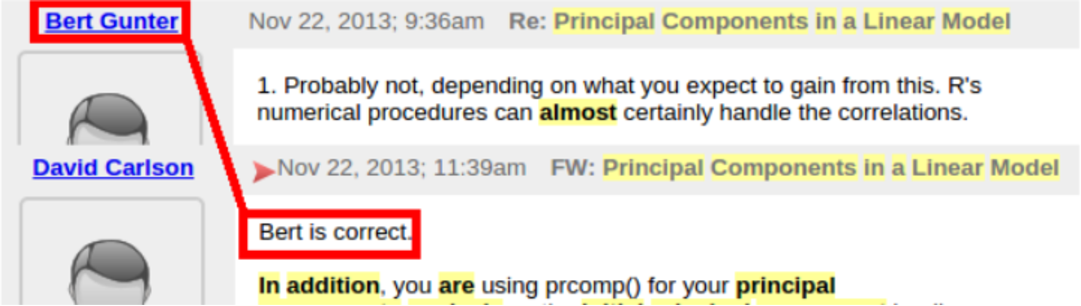
\includegraphics[width=\columnwidth]{../Figures/ML-PKimg2}
        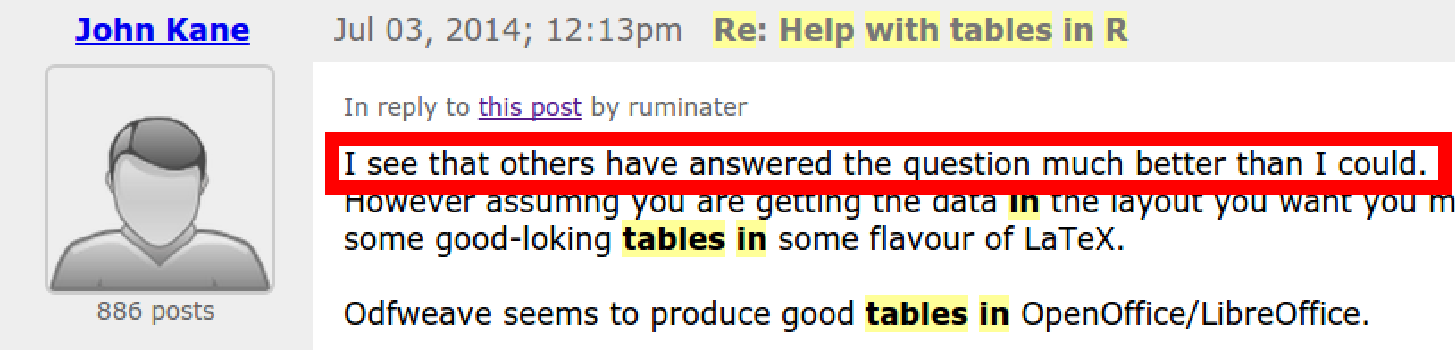
\includegraphics[width=\columnwidth]{../Figures/ML-PKimg11}
        \caption[Participatory knowledge construction on the \RH mailing list.]{Participatory knowledge construction on the \RH mailing list.}
        \label{fig:ML-PK1}
          \end{figure}

On \SO, \textit{participatory knowledge} construction takes place when:
    \begin{enumerate*}[label=(\arabic*)]
    \item one can infer a link between answers, through either a direct or indirect reference; or
    \item comments complement the answer or directly cite another author.
    \end{enumerate*}
Participatory knowledge construction also occurs in different places on \SO, perhaps as a consequence of its rich interface. We observe this type of knowledge construction when a user answers a question and directly cites or links to someone else's answer in the thread, or when a user cites someone else's question or answer in a comment (a typical case is linking to a previously asked question). Figure \ref{fig:SO-PK1} depicts an example of participatory knowledge construction on \SO: when an answer was deemed insufficient, a user helped out by adding a comment and referencing another author's answer.

    \begin{figure}[!htb]
        \centering
        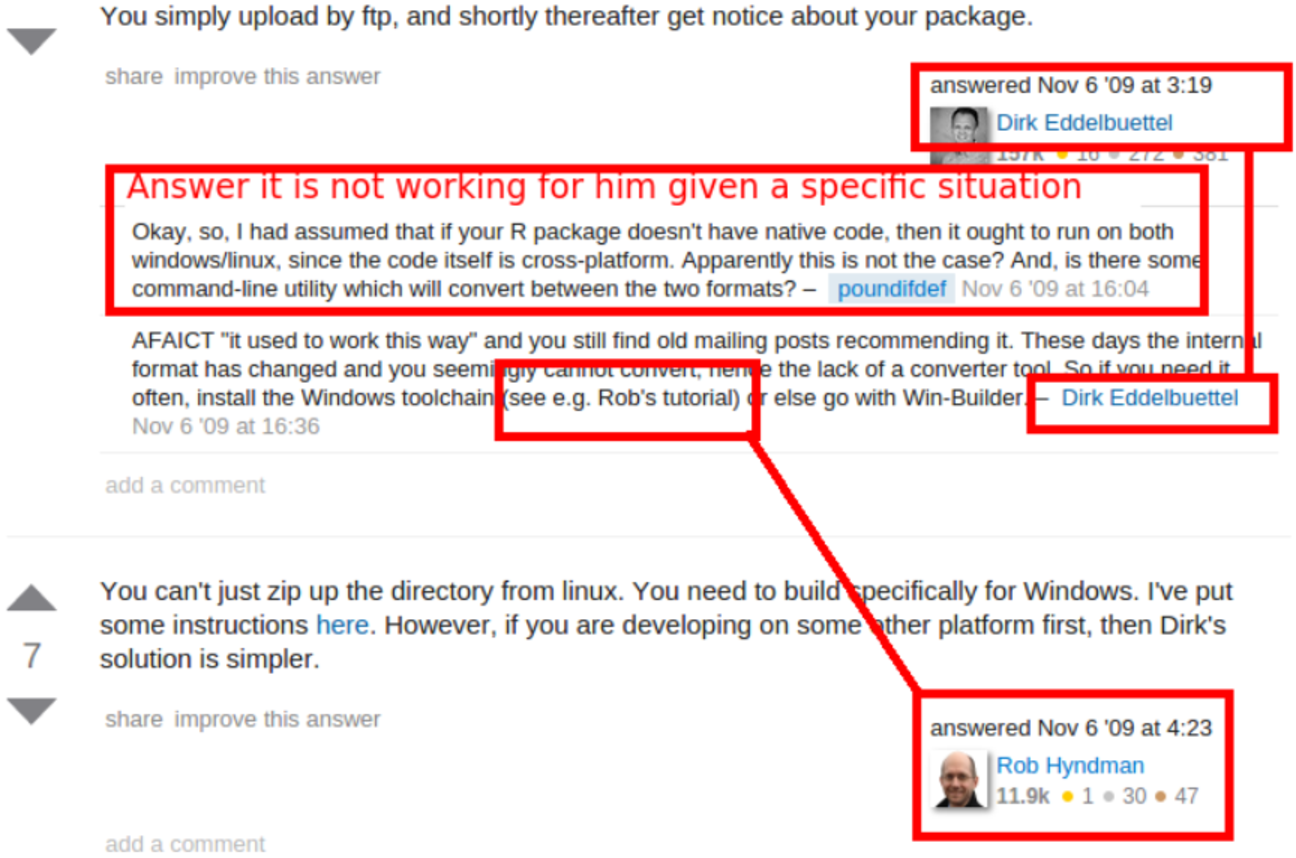
\includegraphics[width=\columnwidth]{../Figures/SO-PKimg5}
        \caption{Example of participatory knowledge on \SO. Users built on the comments and answers of other users.}
        \label{fig:SO-PK1}
            \end{figure}

On the \RH mailing list, we observed \textit{crowd knowledge} construction when different messages responded directly to the original question, rather than to another response.

On \SO, \textit{crowd knowledge} construction is observable when:
  \begin{enumerate*}[label=(\arabic*)]
    \item there is no direct or inferable reference between answers; or
    \item an answer is a variation of one of the other answers on the thread.
  \end{enumerate*}
Figure \ref{fig:CKC_MLSO} depicts an example of crowd knowledge construction on \SO. As can be seen from the figure, two of the three answers provided the same solution. 

    \begin{figure} [!htb]
        \centering
        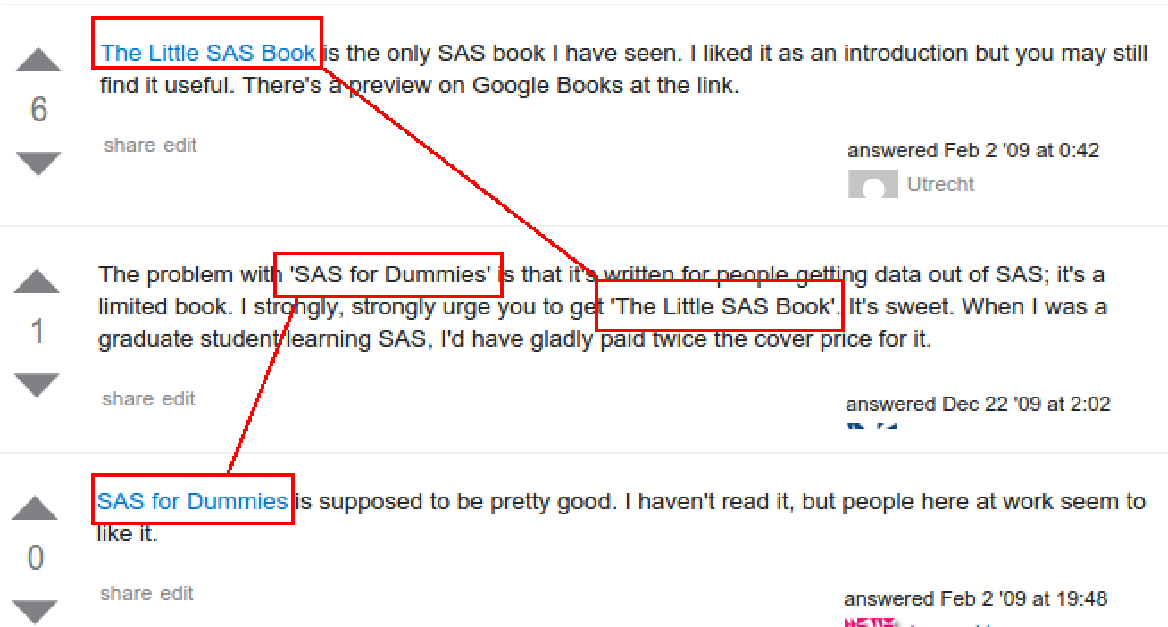
\includegraphics[width=\columnwidth]{../Figures/SO-CSimg2}
        \caption{Example of how crowd knowledge construction occurs. The three authors provided similar answers, but did it independently of each other.}
        \label{fig:CKC_MLSO}
    \end{figure}

% RQ3
\subsection{Why Users Post to a Particular Channel or to both Channels}
From our survey, we were able to learn why some R community users preferred one channel over the other. We summarize their responses below. Using results from the analysis of the archived data, we then present why some users post some questions to both channels. 

\subsubsection{Why Participants Post on \SO}

Survey participants preferred using \SO for several reasons: (a) the ability to gain peer recognition (the advantage of gaining points---and visibility---is a major draw of \SO); (b) its rich and user-friendly interface; (c) answers are straight to the point; (d) questions are usually answered faster on \SO than on the \RH mailing list; and (e) it is easy to search for previous questions and answers.

However, the respondents reported a few main drawbacks of using \SO: (a) there is an overabundance of related questions; (b) one requires a certain level of experience to understand some of the answers; and (c) \SO's strict rules only allow questions and their answers, they do not allow discussions nor questions about opinions.


\subsubsection{Why Participants Post on the \RH mailing list}
\label{sec:rh}

Survey participants reported a few benefits of using the \RH mailing list: (a) the email format is convenient; (b) following the mailing list provides awareness and increases learning in new topics; (c) there is more flexibility regarding the topics that one can discuss; and (d) there is much participation from highly experienced users. The respondents did note a couple of disadvantages of \RH: (a) some discussions lead to aggressive behavior; and (b) searching the archives is not easy.

\subsubsection{Why Participants Post to Both Channels}

Our analysis of the archived data revealed that some users (79 cases in our sample) posted the same question on both channels. 
Based on the responses from the survey, we identified that being active on both channels brings benefits to those asking and answering questions (RQ3).

\begin{description}[itemsep=2pt, topsep=0pt, leftmargin=1em, parsep=0pt]
\item[Find a better answer:] As expected, two channels are better than one---
  one channel might result in a better answer than the other.
\item[Support follow-up questions:] We found that the \RH mailing list is often used to conduct follow-up discussions on
  specific answers provided to \SO questions. \SO's focus is on finding an answer to a question and does not
  provide an environment to discuss the specifics of an answer (unless it is asked as another question).
In contrast, a discussion on \RH can continue long after an answer has been found through follow-up questions, and not only by the person who asked the original question.  
\item[Speed up answers:] users ask the same question on both channels in order to get an answer faster. However, this behavior is not encouraged by the community as it is deemed impolite\footnote{\href{https://goo.gl/p9vVaj}{https://goo.gl/p9vVaj}}.
\end{description}

%RQ4. How does participation differ between the two channels over time?
\subsection{\rqd}

To bring insights to RQ4, we first discuss how user participation differs between the two channels over time and then consider how long users participate. 

\subsubsection{How user participation differs
between the two channels over time}

In their research, Vasilescu et al. studied the participation of the \RH and \SO communities over time. Their
research showed strong evidence that knowledge seeking activities were moving from \RH to \SO---as of the end of
2013~\cite{Vasilescu2014c}.
Their findings findings prompted us to also consider how participation differs over both channels over time (RQ4).  We first explore the evolution of the number of questions in both channels, as the main proxy of activity. The results
are shown in Figure~\ref{fig:channelsActPerMonth}. As reported in~\cite{Vasilescu2014c}, the trend indicates that \SO
continues to grow and \RH continues to decrease. One aspect that is changing in \SO is the growth of questions that
receive an overall negative score. A score in \SO is the sum of positive votes minus negative votes and can be seen as a proxy of
the quality of the question. As can be seen, the number of questions with an overall positive score has flattened and is starting to decrease.

However, looking at the trends over the last 10 years, this might be misleading. Figure~\ref{channelsActPerMonthLatests} shows only the
number of questions since Jan 2015. As can be seen, both channels are relatively flat in terms of overall questions. The
number of questions in \SO is between 10 and 20 times the number of questions in \RH, but the number of questions with
a positive overall score in \SO is starting to decrease (we recognize this might be a temporary effect).

\begin{figure*}[htbp]
  \centering
  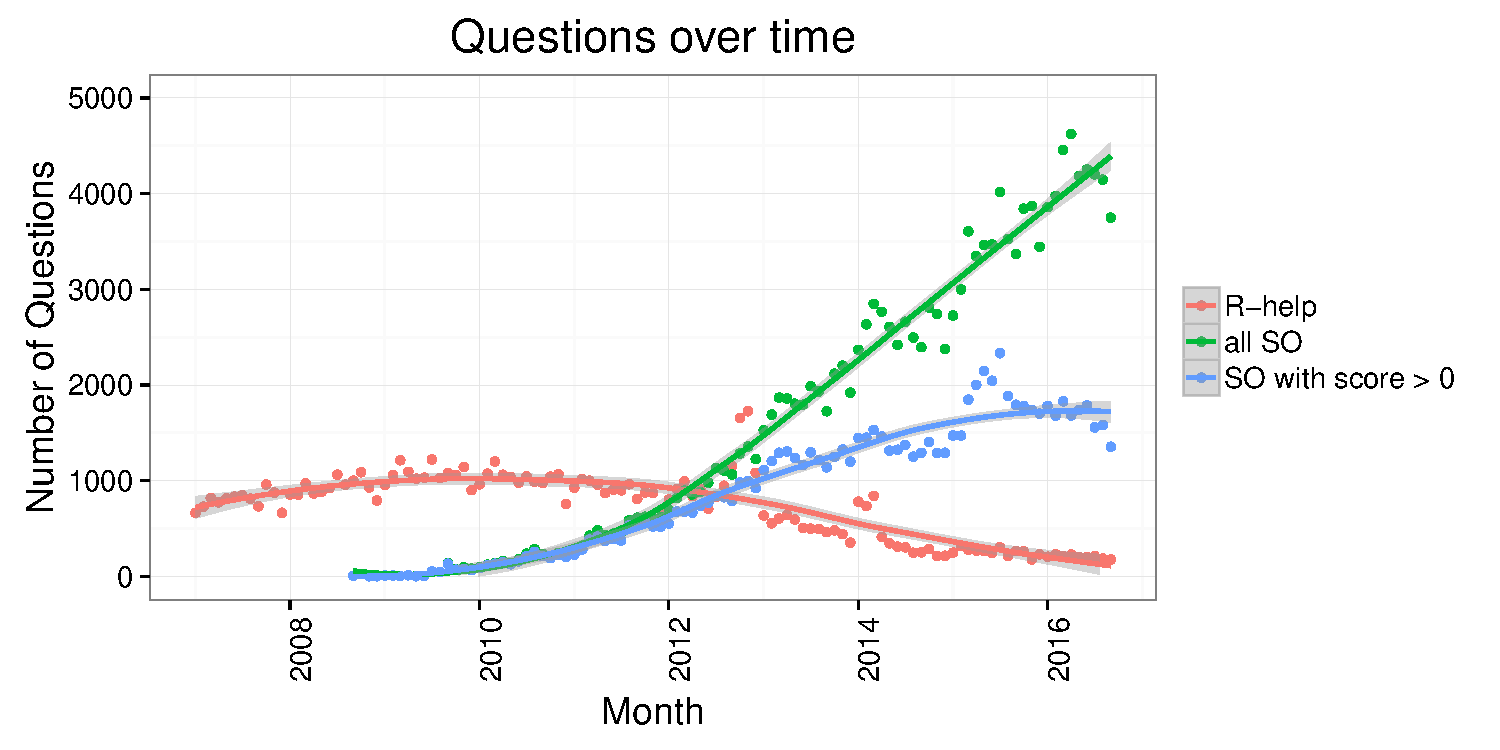
\includegraphics[width=.95\textwidth]{figs/actByMonth.pdf}
  \caption{Number of questions asked over time. As can be seen, \SO activity has been much larger than \RH. However,
    the number of questions with positive score has flattened.}
  \label{fig:channelsActPerMonth}
\end{figure*}


\begin{figure*}[htbp]
  \centering
  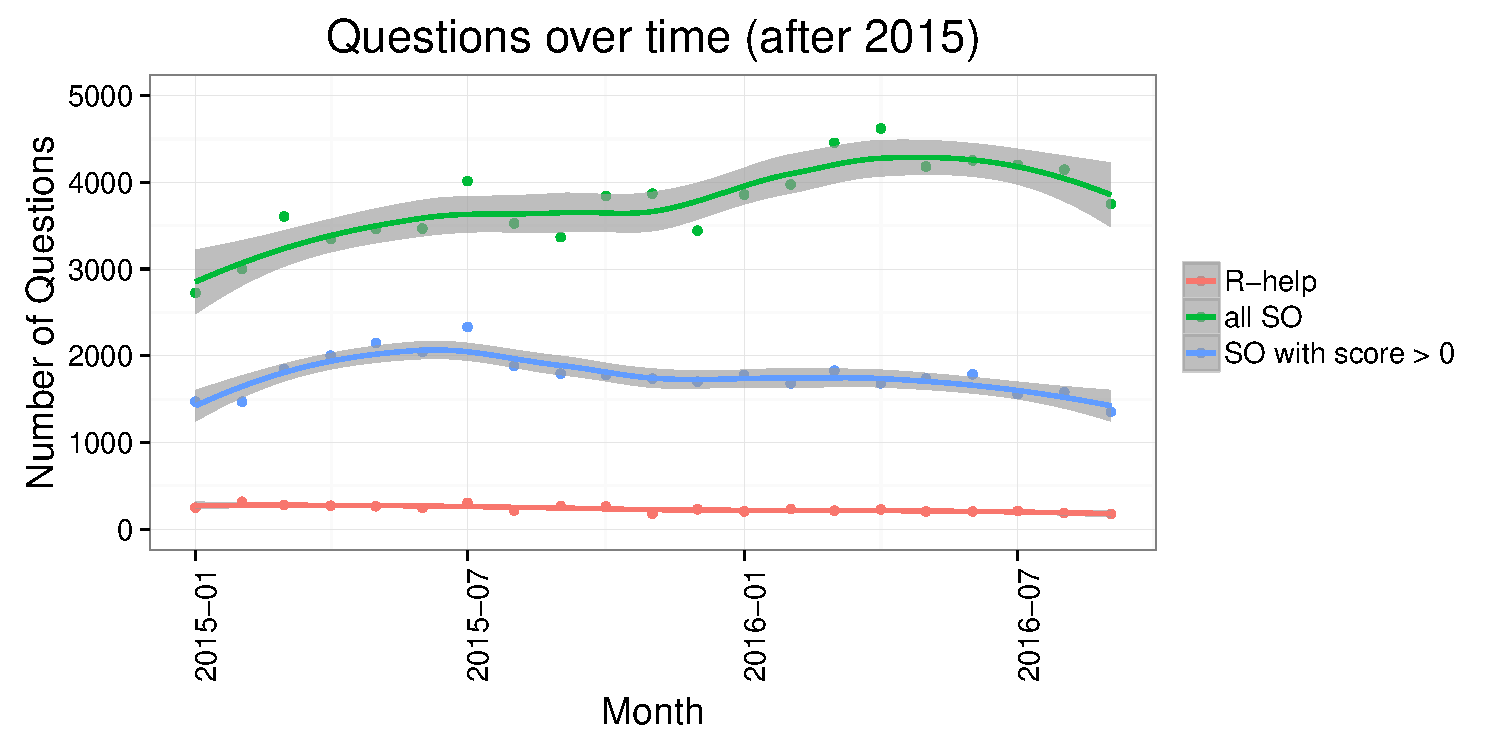
\includegraphics[width=.95\textwidth]{figs/actByMonth2016.pdf}
  \caption{Detail of Figure~\ref{fig:channelsActPerMonth} showing only activity after January 2015. As can be seen, both
    channels have flattened, but the number of questions with positive score in \SO is starting to decrease.}
  \label{fig:channelsActPerMonthLatests}
\end{figure*}

\subsubsection{How long users participate}

Another important measure of the community and its ability to curate and maintain knowledge is if their users continuously participate
over time, even if their participation is small. To measure the continuity of participation in both
channels, we divided the history of both channels into one month segments. In \RH, we considered that a user participated in a given month if they
posted at least one email to the list during that period. For \SO, we considered that a user participated in a given month if they
posted, responded to, or commented on at least one question.

The results show that users do not participate in either channel for a long
time. Figure~\ref{fig:monthsPerUser} shows the accumulated proportion of users that participate during a given number of
months (not necessarily consecutively). The curves are very similar and skewed: 62\% of \RH users and 65\% of \SO users are active one month only, and
90\% of \RH users are active 5 months or less, while in \SO, 90\% of users participate 4 months or less.

\begin{figure*}[htbp]
  \centering
  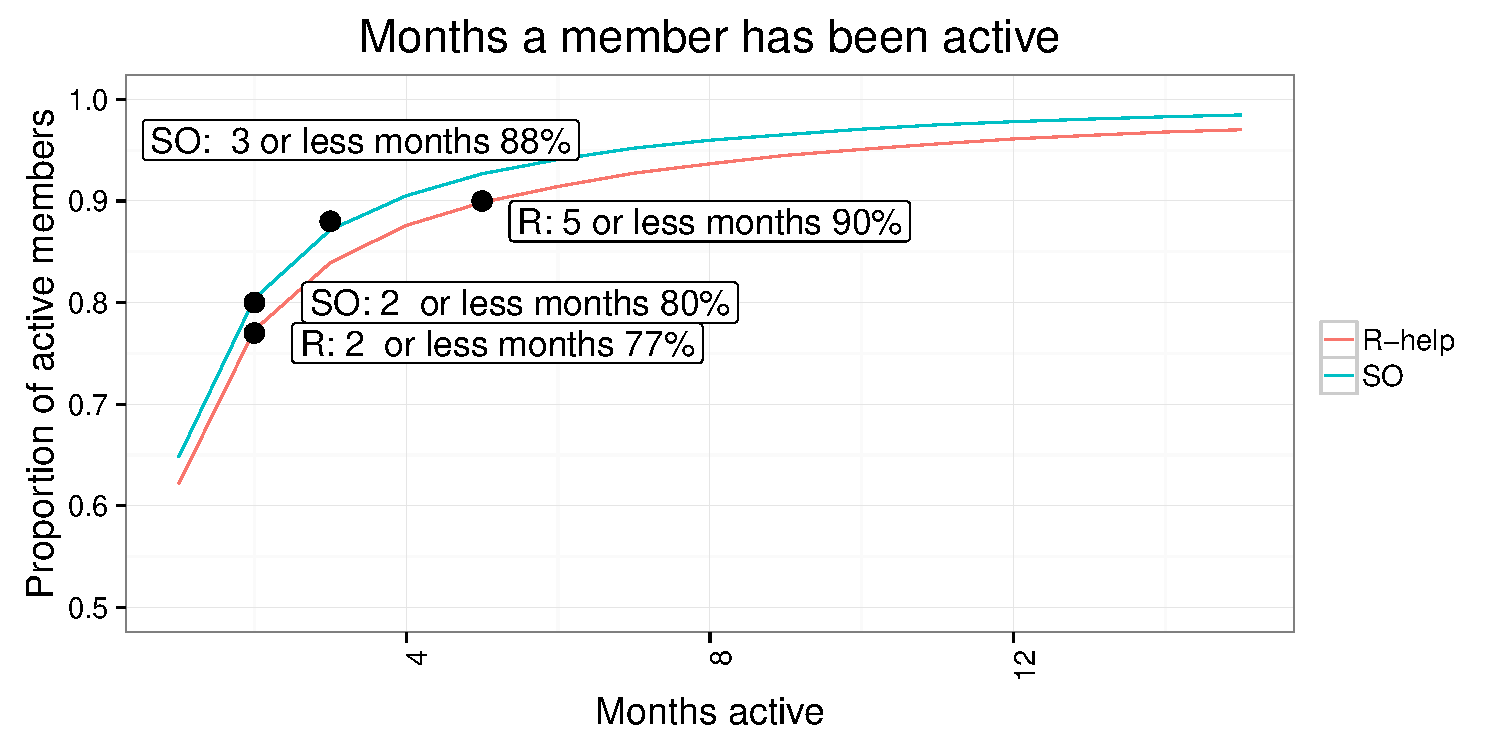
\includegraphics[width=.95\textwidth]{figs/monthsPerUser.pdf}
  \caption{Months a user has been active. This plot shows the accumulated proportion of users who have been active at a
    given number of months. As can be seen, 62\% of \RH users and 65\% of \SO users are active one month only.
    90\% of \RH users are active 5 or less months. In SO, 90\% of users participate 4 or less months. Months do not have
  to consecutive.}
  \label{fig:monthsPerUser}
\end{figure*}



%RQ5. Are there significant differences in participation activity between community users?
\subsection{\rqe}

To consider participation activity of members in the two channels, we first consider new users. We wish to explore, how many newcomers there are to both channels, and we consider if they are likely to post again.  Lastly, we look at contributors that are responsible for the vast majority of posts in both channels.


\subsubsection{Amount and the follow up activity of new users}

New users are important for the survival and continuity of a community. Unfortunately we can only track users when they
participate in a channel, so we do not know who is a passive participant. Hence we use the date of a first
contribution as the proxy of when a user joins the community.  Figure~\ref{fig:newusers} shows the proportion of users
who have posted their first question in a particular month. As can be seen, both communities show a very similar
pattern: between 25 and 35\% of the users who post new questions are new during that month. We found, however, that many
of these users participate only once: they post a question and they never post anything else, neither a question nor an
answer (see Fig.~\ref{fig:newusersOnce}).  One year after the creation of \SO, around 1 in 10 users
only ever post one question, while in \RH the number has been increasing over time. There has been a visible decrease in
the proportion of new users contributing to both channels.

In fact, the number of users who only participate once (at any time) is relatively large over the lifetime of the channels: 43\% in
\RH and and 32\% in \SO.

\begin{figure*}[htbp]
  \centering
  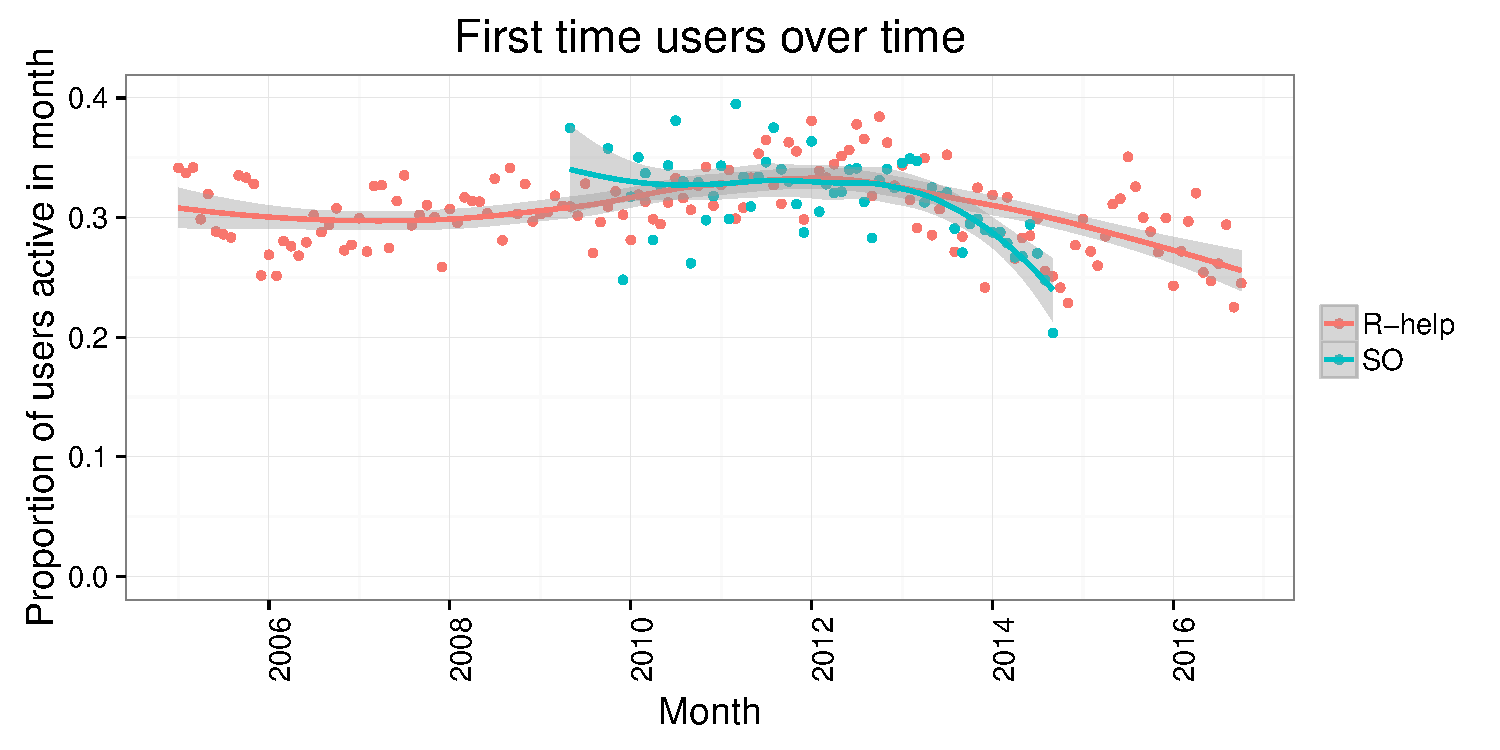
\includegraphics[width=\textwidth]{figs/actByMonthUsers.pdf}
  \caption{Proportion of new users over time. The top lines (thicker) correspond to
    the number of users who post their first question in that month.
The bottom (thinner) lines  correspond to the subset of new users who only ask one
    questions and never participate again. }
  \label{fig:newusers}
\end{figure*}

\begin{figure*}[htbp]
  \centering
  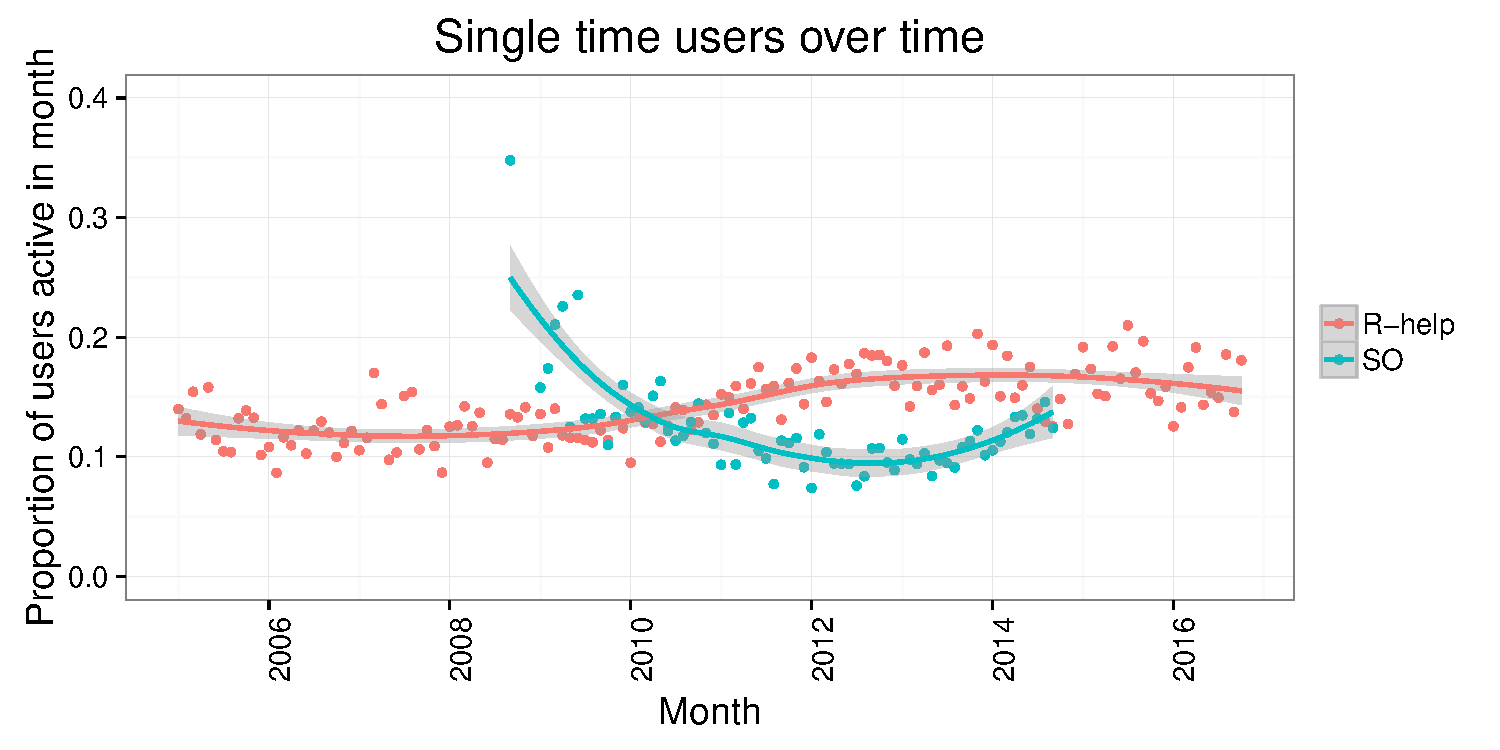
\includegraphics[width=\textwidth]{figs/actByMonthUsersOnce.pdf}
  \caption{Proportion of one time users in any given month. }
  \label{fig:newusersOnce}
\end{figure*}



\subsubsection{Common users of both channels}

The number of common users between both datasets that we identified is relatively small (around 2.5\% of all
users). Yet, a handful of these contributors are responsible for a very large proportion of the answers in both
channels. Figure~\ref{fig:common} shows the accumulated proportion of answers that have been contributed by these
authors. As can be seen, the top contributor has contributed 3.9\% and 3.7\% of answers in \RH and \SO,
respectively. In fact, the top 6 contributors to both channels are responsible for 10\% of the answers to both. 
Answers to \SO include both posts and comments to questions.

\begin{figure*}[htbp]
  \centering
  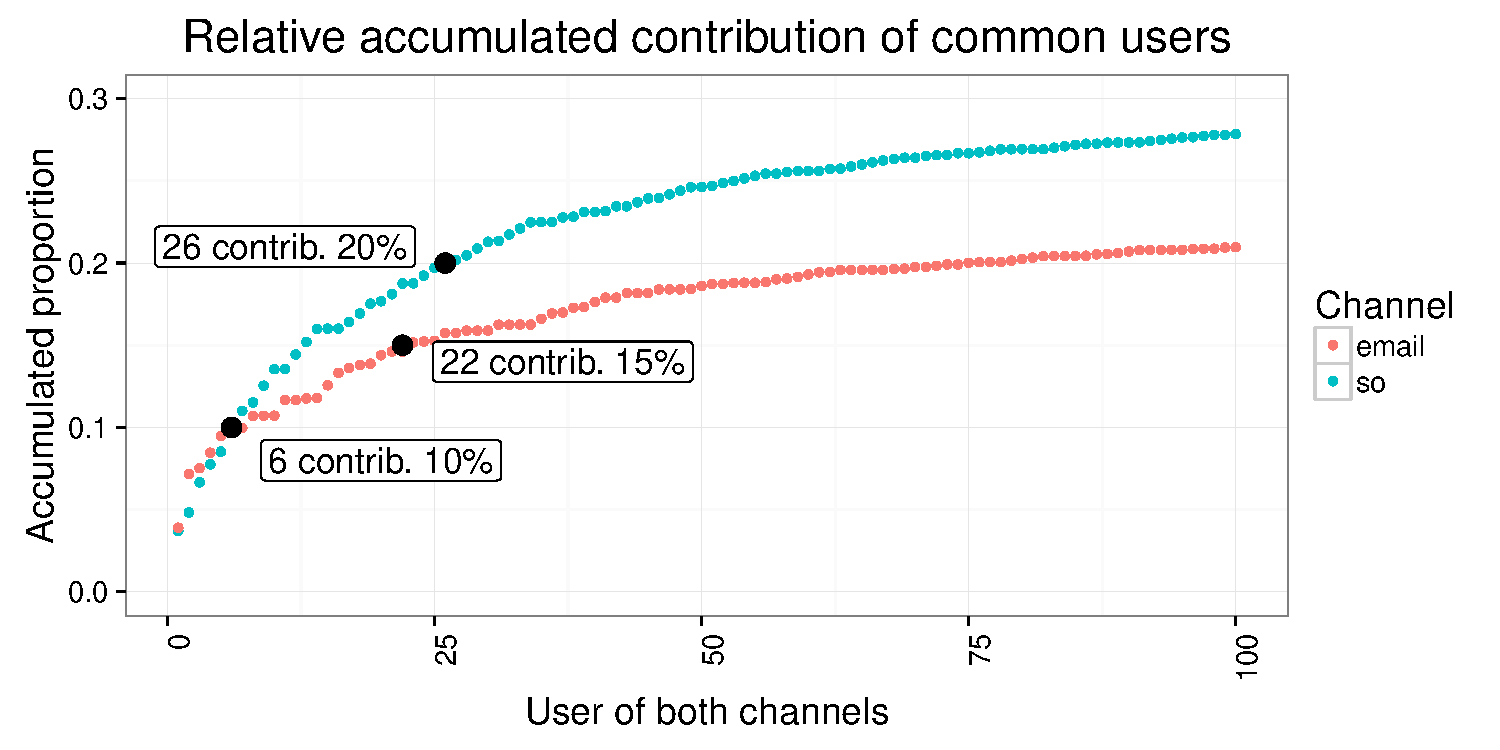
\includegraphics[width=.95\textwidth]{figs/common.pdf}
  \caption{Accumulative proportion of contributions by the most prolific users who post to both channels. As can be seen, the top 6
    most prolific users contribute approximately 10\% of the answers in both channels.}
  \label{fig:common}
\end{figure*}

\subsubsection{Prolific contributors}

Both channels benefit from a handful of very prolific users who answer most questions. Thus, we refer to these users as
\textit{prolific contributors}. Figure~\ref{fig:prolific} shows the prolific contributors in each channel, ordered by the number of
answers they have contributed. The vertical axis shows the accumulated proportion of contributions to all answers in
each channel. As can be seen in \RH, 9 users have contributed 25\% of all answers and 49 have contributed 50\% of all answers. In \SO, the distribution is not as
steep, yet 24 users have contributed 25\% of all answers (including comments) and 131 have contributed 50\% of all answers. This
means that 0.15\% of the \RH mailing list users contribute 50\% of all the answers, while 0.45\% of the \SO users contribute 50\%
of all the answers. To put this into context, the prolific contributors in \RH post between 2 and 3 answers a day on average, while the
prolific contributors of \SO average between 3 and 5 answers a day.

\begin{figure*}[htbp]
  \centering
  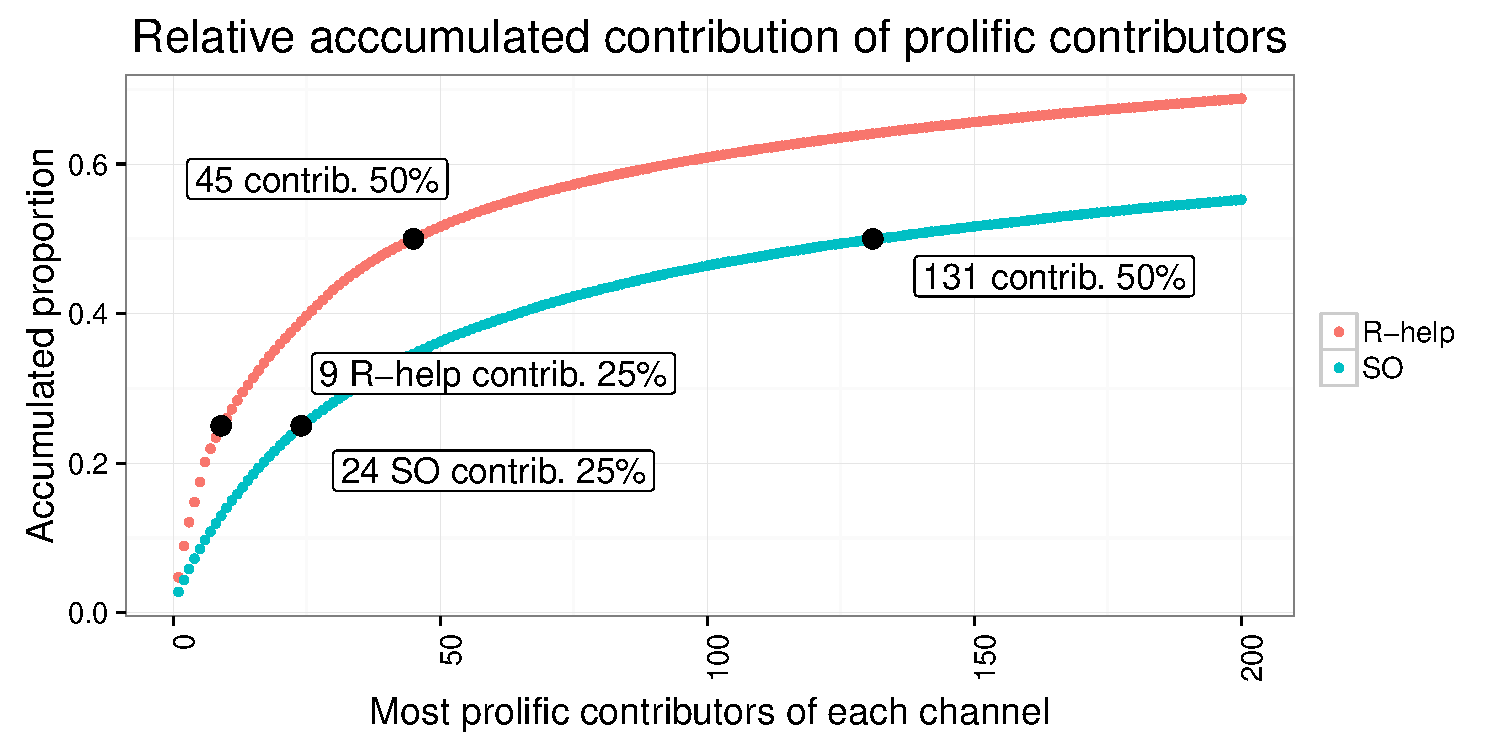
\includegraphics[width=.95\textwidth]{figs/prolific.pdf}
  \caption{Accumulative proportion of contributions by the most prolific users of each channel. As can be seen, the
    top 9 and top 24
    contributors to \RH and \SO, respectively, are responsible for 25\% of all the answers.}
  \label{fig:prolific}
\end{figure*}



\section{Discussion}
\label{cha:theory}

In this section, we reflect on the results presented in the previous section and place them within the context of related research. Additionally, we identify research opportunities and derive recommendations for using multiple Q\&A channels.
In the following, we provide representative quotes extracted from the survey, using P\# to indicate the participant ID.

\subsection{Knowledge Creation and Curation}

    Based on the results, both channels provide similar knowledge support for questions and answers.
    However, there are some important differences between the channels which we discuss in detail below (and summarize in Table~\ref{table:constrat}).

    \begin{table}[!htb]
      \centering
      \caption{Comparison of the way knowledge is shared on \SO and the \RH mailing list.}
      \label{table:constrat}
      \begin{small}
        \setlength{\tabcolsep}{5pt}
        \begin{tabular}{@{}lll@{}}
          \toprule
          \textbf{}      & \textbf{\SO} & \textbf{\RH}\\
          \midrule
          Knowledge construction & Mainly crowd             & Mainly participatory \\
          Topic restriction      & Yes & No \\
          Emphasis & Curating knowledge & Developing knowledge \\ 
          \bottomrule
        \end{tabular}
      \end{small}
\vspace{-4mm}
    \end{table}

\subsubsection{Knowledge construction}

\SO's gamification mechanism encourages users to be first when answering questions~\cite{Singer2013}. In contrast, the \RH mailing list is a less competitive
environment where users tend to build on other responses. On \RH, users work as a team rather than as individuals searching for points (as is the case on \SO).
As a result, knowledge on \SO is built in a more crowdsourced manner, while knowledge on the \RH mailing list is usually built in a participatory manner.

Since, the competitive \SO environment creates an incentive to be the first to answer rather than improve and build on other answers, it is common to find a question with several answers that provide the same information. For example, three of the six answers in the \SO question titled \textit{``Resources for learning SAS if you are already familiar with R''}\footnote{\url{http://goo.gl/Mb4Pbk}} referenced the same books.
And while \SO provides a powerful curation mechanism to ensure the best answers make it to the top, this mechanism does not explain why an answer is better than another.

In contrast, the \RH mailing list tends to be more participatory in how users construct knowledge. It fosters an environment where users discuss proposed answers---users tend to provide more background to answers and explain the rationale behind them.
For example, the question \textit{``Arrange elements on a matrix according to rowSums + short `apply' Q''} was posted to both \SO\footnote{\url{http://goo.gl/a8AES8}} and {\RH}\footnote{\url{http://goo.gl/PGflT5}}. This question illustrates the contrast in how the two communities build knowledge.
On \SO, each participant contributed a solution without any evidence of collaboration with others.
Whereas users on the \RH mailing list complemented each other's answers by providing further information and insights to the answers already
contributed. Vasilescu \textit{et al.}~\cite{Vasilescu2014c} showed that users who are active in both channels tend to provide answers faster on \SO than on \RH,
suggesting that they are motivated by the gamification aspects of \SO, and thus tend to gravitate towards crowd knowledge construction.

    
While prevalent, the construction of knowledge on \SO is not limited to the crowd-based approach. Participatory knowledge construction is also existent, such as by up/down voting questions and by the provision of comments. In most cases, participatory knowledge construction on \SO is used for editing answers (e.g., correcting grammar) or linking to previously asked questions.
Similarly, some knowledge on the \RH mailing list is constructed in a crowd-based manner, but this is less prevalent than participatory construction.

Tausczik \textit{et al.}~\cite{Tausczik2014} examined how users of Math Overflow (a Q\&A platform for mathematicians) collaborate and construct knowledge. They found that collaboration was diverse and fell on the spectrum between \textit{independent} (crowd-based) and \textit{interdependent} (participatory). Similar to our findings with \SO, the most common collaborative act was of an independent nature (i.e., providing information), while other contributions that built on existing work were less common (i.e., clarifying the question, critiquing answers, revising answers, and extending answers).

Our results seem to imply that \SO's gamification features, while highly effective, have the side effect of reducing collaborative knowledge creation between users. In their study on building \SO reputation, Bosu \textit{et al.}~\cite{Bosu2013} proposed six strategies for increasing reputation score, two of which were \textit{be the first to answer}, and \textit{do it at off-peak hours}, indicating crowd knowledge creation. Furthermore, while \SO gives people the ability to vote on comments, it does not reward points to users that post comments. For example, some users search \SO for answers within comments and convert them to proper answers to gain reputation points\footnote{\url{http://duncanlock.net/blog/2013/06/14/the-smart-guide-to-stack-overflow-zero-to-hero}}.


                
\subsubsection{Topic restriction}

\SO's participation rules only permit questions that have a clear answer, making it topic restrictive. In contrast, the \RH mailing list is suitable for discussing
any topic related to the R language. For example, questions related to R but not focused on software development are not rejected by the \RH mailing list community---topics that trigger discussion are welcomed.

\SO questions that trigger a discussion are flagged as opinion-based or off-topic and typically closed. Correa and Sureka~\cite{Correa2014} found that 18\% of deleted questions on \SO are subjective (i.e., ask for opinion).
For example, a question titled \textit{``What's a good example of really clean and clear [R] code, for pedagogical purposes?''}\footnote{http://goo.gl/9JjZW1} was flagged as \textit{off-topic} because the question was not related to software development.
An \RH user wrote a fine explanation of the purpose of each channel in a message on the mailing list:\footnote{\url{http://goo.gl/mTccwx}}
    \begin{quote}
        \textit{``Got an R programming question that you think has a definite answer? Post to [\SO]. Want to ask something for discussion, like what options there are for doing XYZ in R, or why lm() is faster than glm(), or why are these two numbers not equal? Post to \RH. Questions like that do get posted to [\SO], but we [vote] them down for being off topic and they disappear pretty quickly.''}
    \end{quote}

Squire reported that, despite the gains in participation and the response time provided by \SO, many development communities keep using mailing lists, either as
a primary communication channel or as part of a hybrid solution where multiple channels are used, thus allowing for non-restrictive topics and fostering of
discussion~\cite{Squire2015a}.
Mailing lists are also favored for their simplicity, and for allowing guaranteed delivery (i.e., knowing who will receive the email) ~\cite{Zhang2015}.

        
\subsubsection{Curated knowledge and knowledge development}

One of the main benefits enabled by \SO's crowd-based knowledge construction is the creation and curation of a pool of questions and answers. In contrast, \RH provides an environment in which users
    develop knowledge through participation, but this knowledge is not curated for future use. This makes the information difficult to be reused by those who were not
    participants (either active or passive) during its creation.


            While \SO has been successful, some users feel that by not fostering discussion, it restricts thinking that might lead to better answers, as P26 explained:
    \begin{quote}
        \textit{``Many developers share my view that [\SO] is a very bad model, ... [it] removes the value added by reading list traffic that doesn't seem directly relevant to a currently conceptualized question, but which may lead to a new conceptualization (out-of-the-frame thinking). [\SO] cannot do that.''}
    \end{quote}
    Similarly, P35 stated that they use the \RH mailing list if the questions are not 100\% \textit{``help-me-to-code-this''}.

    However, \SO shines when questions have to be kept for posterity. 
    Its curation mechanisms provide tools for keeping the channel clean of what seems to be unnecessary information (e.g., flagging questions, deleting comments, editing messages, and demoting irrelevant answers), as P14 explained:

    \begin{quote}
        \textit{``[\SO] is an excellent model for providing a rich resource for users of R, which the \RH mailing list was not. 
        Ability to include light markup, render code blocks nicely, no nested email threads all helps the experience of searching for and finding the help that a user needs, and I want to contribute to that.''}
    \end{quote}

        
\subsubsection{Research opportunities}

An important research question that arises from these findings is whether \SO's model can be improved to provide better participatory knowledge construction support without hindering its ability to curate information for future use.

Another interesting aspect emerging from our findings is that the activity on the \RH mailing list is only marginally smaller than on \SO (the proportion of responses in each category fluctuated between 1.4 and 2 times). Further research is required to assess and verify the quality and effectiveness of answers.

\subsection{Recommendations for Using Multiple Q\&A \Channels}



One of the expected outcomes of this study is a set of recommendations for using multiple \channels. Other research on \SO also points to these and other recommendations.  For example, Yao \textit{et al.} discuss the importance of how the phrasing of a question influences the quality of the answer provided~\cite{Yao2013a}, and Anderson \textit{et al.} emphasize the importance of badges (gamification) on participation~\cite{Anderson2013}. In the following, we build on the existing literature as well as our results to  provide five recommendations for people seeking or contributing answers.  Our recommendations are summarized in Table~\ref{tab:recom}.



    \begin{table}[htbp]
      \caption{Recommendations to improve the benefits from using several Q\&A channels.}
      \centering
\small
      \begin{tabularx}{1.0\linewidth}[h]{@{}X@{}}
          \toprule
\reca \\
\recb \\
\recc \\
\recd \\
\rece \\
          \bottomrule
      \end{tabularx}
      \label{tab:recom}
    \end{table}




\subsubsection{\reca}


    Each channel provides a list of \textit{topics} that are deemed acceptable.
    The topics are regulated either by the community or the channel's moderators. \textit{``...\SO has (a) more limited range of help topics (help for code only), whereas \RH is broader (philosophy, posting announcements, etc.)''} [P35].
    Knowing which channel is more suitable for a specific topic can improve the response time or the quality of the answer.


    In some cases, it is expected that questions will be answered by a \textit{specific group} (e.g., R-core team) regardless of the topic, as P32 stated: \textit{``If I really want an answer from someone in R-core or closely related people, I would definitely choose the mailing list.''}
    For example, in the \RH thread \textit{``Co-integration and ECM in Package \{urca\}''}\footnote{\url{http://goo.gl/7olLv7}} a participant asked the R-core team how to solve a problem: 
     \begin{quote}
     \textit{``Dear R Core Team, I am using package \{urca\} to do co-integration and estimate ECM model, but I have the following two problems...''}
     \end{quote}
    In this scenario, Websites associated with a specific package or library might be the best way to communicate directly with the creators of that technology. Thus, the \RH mailing list is a place for discussion and \SO is a place for questions that have a clear answer.

     





\subsubsection{\recb}

    Throughout this study, we noticed that most of the harsh responses were given to users who did not learn the participation rules or had not learned the basics of R or statistics.
    For anybody using a channel, the community expects users to familiarize themselves with the channel in advance and learn the basics of the technology that they are discussing.

    
    \SO provides user guides\footnote{\url{http://stackoverflow.com/help}} for each of the main features of the channel, such as badges, questions,
    answers, flags, comments, and the reputation system. The \RH mailing list only has general instructions\footnote{\url{https://www.r-project.org/mail.html\#instructions}} and a guide about posting on the channel\footnote{\url{https://www.r-project.org/posting-guide.html}}.

We also discovered that the R community has developed resources to improve the quality of participation on the communication channels.
    For example, the post on \SO \textit{``How to make a great R reproducible example?''}\footnote{\href{http://stackoverflow.com/questions/5963269/how-to-make-a-great-r-reproducible-example}{http://stackoverflow.com/questions/5963269/how-to-make-a-great-r-reproducible-example}} provides tips and tricks for creating a reproducible example using the R language.
    Another example is the document \textit{``How to write a reproducible
      example''}\footnote{\url{http://adv-r.had.co.nz/Reproducibility.html}} which provides tips for posting a reproducible R code example to mailing lists: \textit{``...Before putting all of your code in an email, consider putting it on \url{http://gist.github.com/}{[GitHub Gist app]}. It will give your code nice syntax highlighting, and you don't have to worry about anything getting mangled by the email system...''}

    Finally, there are manuals like \textit{``An Introduction to R''}, and the FAQ Web pages for R that are available to the public---most of the time, free of charge---and from which any user can learn the basics of R.
    For example, the R community provides a compendium of PDF documents for new users of different languages.\footnote{The R manuals are available at \url{https://cran.r-project.org/}}
    In \SO, supported technologies are provisioned with Web pages and links to free and paid materials.\footnote{Materials available at \url{http://stackoverflow.com/tags/r/info}}
    


\subsubsection{\recc}

    In spite of reading the documentation, a user may fail to address the channel appropriately.
    The community may feel that the question asked, the information provided, or something else entirely is not in compliance with the expectations and rules of the channel.
    In such cases, one should describe the documentation read, the attempts made, and the goal(s) they want to achieve.
    This would avoid answers like \textit{``read the manual''} or \textit{``read the posting guide''}.     For example, in the thread \textit{``lme4 GLMM''}\footnote{\url{https://goo.gl/Gbek3R}} the user explicitly acknowledged the repeated question and explained the rationale for doing so: \textit{``I'm very sorry for my repeated question, which I asked 2 weeks ago, namely: I'm interested in possibly simple random-part specification in the call...''}


\subsubsection{\recd}

    A common practice to answer or ask questions is to provide links for documentation, examples, source code, or other resources.
    As links point to online resources that might not exist in the future, it is important to include the key points of the resource within the question or answer.
    For instance, when a question or answer contains information in an external file hosting service like Dropbox or Google Drive, the owner of the service account can remove or break the link at any moment, leaving the message incomplete or impossible to reproduce.     P33 suggested that \textit{``Questions should be self-contained as much as possible. Exceptions: recognizable links such as CRAN, R documentation, etc.''}

    Based on our observations, we provide the following set of recommendations for using third-party resources within links.

    \begin{description}[itemsep=3pt, topsep=2pt, leftmargin=1em, parsep=0pt]
        \item[Use well-maintained Websites] that are expected to be available in the future, such as Wikipedia and the official documentation in CRAN.
        For example,         a user on \SO posted: \textit{``I'm doing a simulation where I need to calculate a \href{https://en.wikipedia.org/wiki/Convolution_of_probability_distributions}{[Wikipedia link] convolution} of
          \href{https://en.wikipedia.org/wiki/Multinomial_distribution}{[Wikipedia link] multinomial distributions}...''}

        \item[Use resources that support or expand the message] to further clarify the message for those who might need it. For instance, a thread on \SO titled \textit{``How do I save all the draws from a MCMC posterior distribution to a file in R''} states \textit{``...You should be able to open a text connection using ?file \href{http://stat.ethz.ch/R-manual/R-devel/library/base/html/connections.html}{[more information]} with the open argument set to write...''}

        \item[Use links rather than large attachments] as it is not always practical to include all the related information in a message. Providing links to  videos or large documents is usually preferred over including them as attachments.
        For example, in the \RH thread \textit{``Using FUNCTION to create usable objects''}, a user linked to a PDF rather than quoting it: \textit{``I suspect you are trying to find your way
          into Circle 6 of `The R Inferno' but haven't yet got in. \href{http://www.burns-stat.com/pages/Tutor/R\_inferno.pdf}{[link to PDF of R Inferno]}.''}
    \end{description}

\subsubsection{\rece}
\label{sec:userbeh}

It is obvious that users help others by answering questions. However, while analyzing questions and answers, we identified positive user behaviours that
we believe are worth mentioning.  These behaviours provide evidence of an altruistic way of thinking and the strong commitment that users have towards building knowledge in their community.

\begin{description}[itemsep=2pt, topsep=0pt, leftmargin=1em, parsep=0pt]
\item[I answered my own question:] Some questions are answered by the user that asked the question. They posted back to the channel to document their solution and help others: \textit{``Just for the records (and if anyone ever wants to find the `solution'), I solved my own problem.''}\footnote{\url{https://goo.gl/r3z0DX}} 
 
\item[I did it for you:] When answering, authors provide source code to help others: \textit{``I coded up the algorithm from the Cameron and Turner paper. Dunno if it gives exactly the same results as my (Splus?) code from lo these many years ago...''}\footnote{\url{http://goo.gl/GXWGG3}}.

\item[Updated or continued years later:] Some questions are answered months or years later.
For example, a user on \SO modified an answer to provide a more updated version of the source code\footnote{\url{http://goo.gl/k6ZARR}}, and a {question asked on the \RH mailing list in 2012 was continued two years later.}\footnote{\url{http://goo.gl/kgSHZv}}

\item[Ideas to improve the channel:] This behaviour is specific to the \RH mailing list. Sometimes users suggest modifications or new features to improve the channel. For example, a {user proposed to create a package repository that can be accessible through a public wiki or version control interface.}\footnote{\url{http://goo.gl/p0IunD}}
\end{description}

\subsection{Quantitative participation}

In the following, we discuss the implications of the results of the quantitative analysis of users and their
participation in both channels.


\subsubsection{Activity in \SO is slowing down and has stabilized in \RH}

One of the major discoveries of the quantitative analysis of participation over time is the slowing of the growth of
participation in \SO. In particular, that the number of questions asked with an overall positive score is starting to 
decrease over time. This was expected: most frequently asked questions have probably been asked already.  Given the
very large number of questions already asked in \SO, many questions today are expected to be either duplicates of previous
questions, be questions of low intrinsic value (too specific to be useful to others), or end up being flagged as
not a question. 

When we consider that the popularity of R continues to increase, this also implies that new users of R might not need to
post questions to find the answers they are looking for (a testament to the value of the knowledge currently gathered by
\SO). This result also seems to imply that the activities of \SO contributors are shifting from answering new question to
tagging and flagging questions  (e.g. as  duplicates, unclear, or off-topic).

The frequency of postings on the \RH mailing list has now flattened to approximately 200 questions every month. It is possible that
\SO, by reducing the number of frequently asked questions posted on the \RH mailing list, has contributed to a reduction in traffic and
might now be able to concentrate on higher-level questions than those asked in the past. Further research should verify
this hypothesis.


\subsubsection{Frequency of Participation}

Regarding the frequency of participation of users we found that approximately 43\% of users of \RH only ask a question
once (and never participate again, either asking another question, or answering one). In
\SO, the proportion is 33\%. It is not clear why persons will participate once, and further research is needed to
understand why these users do not continue to participate. Similarly, approximately two thirds of users in both channels
only participate during one month and never come back. We have observed in the set of common users that some of them
migrate from one channel to the other. But the majority simply stop participating. It is very likely that they continue
to use \SO as passive users; hence, benefiting from the channel but without contributing back.

Nonetheless, new users appear to be joining both channels all the time. Between 25\% and 35\% of users in any given month
are new. It is very likely that some of them will participate for a long time, guaranteeing the long term survival of
both channels.

\subsubsection{Prolific contributors}

There is a handful of users that are responsible for a large proportion of answers. In \RH, we found that 50\% of the
answers have been contributed by 0.15\% of the users. While in \SO, 0.45\% of the users have contributed 50\% of the answers. It is
not clear if the success of both channels can be attributed to them or not. It is possible, for example, that without
them, other users might have answered those questions. Further research should look into the motivations of these
individuals, the time they commit to help others, and also compare these patterns of activity with similar channels and
see if this is a common phenomenon.

Several of these prolific contributors actively participate in both channels. The top one is responsible for almost 4\% of
the answers in either channel. Combined, the top 6 contributors have authored approximately 10\% of the answers of
either channel. These prolific contributors are very likely serving as a bridge of knowledge between the channels, moving
it from one channel to the other.


\subsection{Threats to Validity}
\label{cha:threats}
Here we examine and discuss threats to the validity of our approach~\cite{Runeson2012}.

\begin{description}[itemsep=3pt, topsep=2pt, leftmargin=1em, parsep=0pt]

\item[Construct validity:] To reach the emerging themes, we relied on subjective human judgment during the data coding
  phase. Researchers had to decide if a message fell within a specific coding category. To alleviate this issue, two
  researchers coded the qualitative data as part of the analysis process. We applied the Cohen Kappa coefficient on
  categories that were not mutually exclusive, but whose purpose was to trigger discussion between coders. We set a
  threshold of 0.8 as the minimum to obtain agreeable results, which is higher than the 0.6 suggested in the
  literature~\cite{Landis1977}.

\item[Internal validity:] \SO's data is structured while the \RH mailing list consists of unstructured data. As a
  result, some of the mapping between the two channels was straightforward (e.g., a follow-up to a reply is a comment to
  that question), while in other cases it wasn't as obvious (e.g., identifying some emails as questions). To reduce the
  risk of bias when mapping the messages between channels, two researchers performed the mapping.

\item[External validity:] Our case study was exploratory in nature and we purposefully aimed to study the R
  community. Many R users are likely to be \textit{casual developers} with limited or non-existent programming
  experience, with backgrounds that vary from biology to statistics. Thus our findings may not apply to other developer
  communities. However, since \SO and mailing lists are widely used by other communities, we believe that our findings
  may be extended to these communities as well~\cite{Squire2015a}. We do not claim the generalizability of our findings
  to other communication channels (e.g., Slack, GitHub), and further research is required to examine how knowledge is
  shared on other channels used by developers.

\end{description}

 \section{Conclusions}
\label{cha:conclusion}

The purpose of this study was to understand how the R community collaborates when using different communication channels in the creation and curation of knowledge.
In particular, we concentrated on studying how this community has used \SO (using the R tag) and the \RH mailing list to both ask and answer questions, through a random sample of 400 threads from each channel. Our research shows that both channels are active communication channels where participants are willing to help others. 

We found that knowledge contributed in response to a question can be classified into four main categories: answers, updates, flags, and comments. The number of
responses sent in each of these categories was between 1.4 and 2.5 times greater on \SO than on the \RH mailing list. While all four types of contributions exist in both
channels, they exhibit differences. For example, on \SO, answers are more focused towards step-by-step tutorials, while \RH answers are more
likely to be suggestions or alternatives. Similarly, on \SO, updates are focused on language (grammar and spelling), while on \RH, the updates are
expansions on previous responses.

The analysis of these questions and answers shows that knowledge is constructed in each channel in a different manner. On \SO, there is a tendency to use
a crowd approach: participants contribute knowledge independently of each other rather than improve other answers. This is likely a result of the
gamification of \SO where the person who provides the best answer is the one that gains the most points.
In contrast, the \RH mailing list uses a participatory approach where participants are more likely to build on other answers, collaborating towards finding the best solution.

Another important difference between both channels is that \SO focuses on making knowledge available for future retrieval. On the other hand, knowledge on the \RH mailing list 
focuses on the discussion of knowledge, but not in its long-term storage or retrieval. Respondents to our survey commented that while it is easy to find answers on \SO
and make sense of them, on \RH it is not only hard to find the relevant answers to a question, but it is also hard to see how the many responses to a question
relate to each other, and ultimately, what the best answer to the question may be.

Another result of our research is that we found that participants prefer \SO to ask questions that are expected to have a direct answer. They prefer to use the \RH mailing list when the
question requests opinions (\SO forbids them) or when they expect to reach core developers of the R project. Some participants ask the same question in both
channels in the hopes of gaining the advantages of both channels. Additionally, \RH has the ability to complement \SO by providing a medium where the rationale
of answers can be discussed.

Overall, this research shows that the R community is committed to using both channels to help others. Each channel has advantages and disadvantages, and the
community appears to be using both effectively to create and curate knowledge regarding the R language.  We provided \textbf{recommendations} for community users that need to use these or other Q\&A channels.  Furthermore, our \textbf{typology of knowledge artifacts} that we summarized in Table~\ref{table:type-of-knowledge} can be used by other researchers that wish to study and understand how knowledge is constructed and curated in other channels or across other communities.  As new channels (such as Slack) become more widely adopted, studying these newer channels and comparing them to existing channels is an imperative aspect of understanding knowledge formation in software development. 












 
\section{Acknowledgments}
The authors would like to thank Cassandra Petrachenko for the editing support and valuable comments that contributed to this work. We also thank Lorena Castañeda for her assistance with the data collection and analysis processes.  Finally, we thank the R community users that responded to our survey.

\bibliographystyle{abbrv}
\bibliography{references}

\end{document}

%%% Local Variables:
%%% mode: latex
%%% TeX-master: t
%%% End:
